\documentclass[
  utf8,%     More capable input encoding than latin-1.
  % parskip,%  For vertical whitespace between paragraphs.  This comes down to more than just using parskip.sty, so it's better to use this class option.
  % S5MP % If you intend to really use margin paragraphs (not recommended!).
%  crop,%     Produce output with crop marks and paper size A4.  Liu-Tryck should like this.  Automatically adds information, including the physical page number, at the top of each page.
       %     Add option 'noInfo' to suppress the info at the top of each page when using option 'crop'.
  % Font options: 'kp' (default), 'times', 'lm'.  The KpFonts (loaded using 'kp'), is the most complete font among the provided options.  Among other, it supports slanted small caps.  See rtthesis.cls for more details regarding the font options.
  largesmallcaps,intlimits,widermath,% Good options to KpFonts.
  sharecounter,nobreak,definition=marks,%  See comments in the results chapter of this document for more information on these options!
  numbers, % If you want to cite references by numbers, use this option.
  noparts% Use option 'noparts' if you do not make use of part divisions.
]{rtthesis}

\usepackage{mythesis}

% !TEX program = pdflatex
% !TEX root = main.tex

\begin{document}
\selectlanguage{english}

\frontmatter
\maketitle

%\begin{abstract}[swedish]
%  Det här som vi har hållit på med är jätteviktigt faktiskt och det vi gjort blev bara sååå bra.  Kanske inte helt otippat, men det glass är sååå gott!

Förresten har vi blivit bäst på att skriva rapporter, så nu ska ska vi inte gå in närmare på några detaljer såhär i sammanfattningen.

%\end{abstract}

\begin{abstract}[english]
  The Equipment Controls and Electronics section (\abbrENSTIECE) at \abbrCERN is developing a high precision piezo-actuated rotational stage for the UA9 crystal collimation project. This collaboration is investigating how tiny bent crystals can help to steer particle beams used in modern hadron colliders such as the Large Hadron Collider (\abbrLHC). Particles are deflected by following the crystal planar channels, "channeling" through the crystal. For high energy particles the angular acceptance for channeling is very low, demanding for a high angular precision mechanism, i.e. the rotational stage. Several control-related issues arising from the complexity and operational environment of the system make it difficult to design a controller that achieves the desired performance. This thesis investigates in different control approaches that could be used to improve the tracking capability of the rotational stage. It shows that the \abbrIRC method could be used to efficiently control the rotational stage. Moreover it shows that a harmonic cancellation method could be used to increase the tracking accuracy by canceling known harmonic disturbances. The harmonic cancellation method (the \abbrRFDC) was implemented in this thesis and proposed as an add-on to the present control algorithm.

\end{abstract}

%\begin{acknowledgments}
  First of all, I would like to thank \abbrCERN and the \abbrENSTIECE section for giving me this opportunity. 

  \addvspace{1em}
  \begin{flushright}
    \textit{%
      Linköping, Augusti 2016\\
      Niklas Ericson%
    }
  \end{flushright}
\end{acknowledgments}


\tableofcontents
\begin{notation}% Passing the option "old" to the notation environment will redefine the notationtabular environment so that it produces an old style LaTeX tabular instead of a ctable.sty style tabular.
  \centering

  % \begin{notationtabular}{Några mängder}{Notation}{Betydelse}
  %   $\naturals$ & Mängden av naturliga tal \\
  %   $\reals$ & Mängden av reella tal \\
  %   $\complexes$ & Mängden av komplexa tal \\
  % \end{notationtabular}

  \begin{notationtabular}{Abbreviations}{Abbreviation}{Meaning}
    \abbrCERN\index{CERN@\abbrCERN!abbreviation} & European Organization for Nuclear Research \\
    \abbrSTM\index{STM@\abbrSTM!abbreviation} & Scanning Tunneling Microscope \\
    \abbrAFM\index{AFM@\abbrAFM!abbreviation} & Atomic Force Microscope \\
    \abbrLHC\index{LHC@\abbrLHC!abbreviation} & Large Hadron Collider \\
    \abbrPEA\index{PEA@\abbrPEA!abbreviation} & Piezoelectric Actuator \\
    \abbrPID\index{PID@\abbrPID!abbreviation} & Proportional, Integral, Derivative (controller) \\
    \abbrDOF\index{DOF@\abbrDOF!abbreviation} & Degrees of Freedom \\
    \abbrPRBS\index{PRBS@\abbrPRBS!abbreviation} & Pseudo Random Binary Sequence \\
    \abbrTF\index{TF@\abbrTF!abbreviation} & Transfer Function \\
    \abbrQFT\index{QFT@\abbrQFT!abbreviation} & Quantitative Feedback Theorem \\
  \end{notationtabular}
\end{notation}


\mainmatter

% !TEX root = main.tex
%en preliminär problemformulering satt i relation till litteraturbasen
\chapter{Introduction}\label{cha:intro}

\section{Background}
High precision positioning systems are vital in e.g. scanning tunneling microscopes (\abbrSTM), atomic force microscopes (\abbrAFM) and in semiconductor lithography. In \abbrAFM, for instance, high precision positioning is required to control the vertical position of the scanning probe to keep the force constant between the sample surface and the probe tip. A topographical image of the sample is obtained by raster-scanning the probe over the sample surface and plotting the vertical displacement against the probe's x-y position. A positioning system that keeps the force constant down to an atomic-scale resolution is thus inevitable in order to obtain a high resolution image without damaging the sample \citep{SurveyOfControlIssues:2007}.

The piezoelectric effect is a phenomenon that arises in certain solid materials when an electric potential is generated in response to applied mechanical stress. The effect was first discovered by Jacques and Pierre Curie in 1880 when they found that applying pressure to a quartz crystal generates electrical potential. Today, the effect is commonly encountered in daily life and utilized in for example lighters, buzzers and loudspeakers.

Smart materials such as piezoelectric and magnetostrictive materials are nowadays commonly used in precision actuators due to their ability to convert electrical energy into mechanical energy. Piezoelectric materials have been commercially available for almost 45 years and have become indispensable for the nanopositioning industry \citep{Piezo:2008}. In cases where a relatively small displacement range is required (travel ranges up to \unit{500}{\micro\meter}) a piezo electric device is the actuator of choice due to its fast response, high resolution and its ability to generate large mechanical forces for small amounts of power in compact designs \citep{SurveyOfControlIssues:2007}.

The \abbrECE (Equipment Controls and Electronics) section in the Engineering Department at \abbrCERN (European Organization for Nuclear Research) is developing a high precision positioning system for use in the UA9 crystal collimation study.

\section{Motivation}
Crystalline solids have the ability to constrain the directions that particles take as they pass through, this is commonly called the "channeling" property. The UA9 collaboration at \abbrCERN is investigating how tiny bent crystals can help to steer particle beams in modern hadron colliders such as the Large Hadron Collider (\abbrLHC) \citep{WebsiteUA9:2016}. In high energy colliders particles tends to drift outwards creating a beam halo. These particles surrounding the beam, can be lost and cause damage to sensitive parts in the accelerator, such as the superconducting magnets which can suffer an abrupt loss in superconducting capability (quench), even from a small dose of deposited energy. To extract and absorb these halo particles, \abbrCERN uses a multi-stage collimation system, consisting of primary and secondary collimators connected in series. \abbrCERN's largest particle accelerator, the \abbrLHC operating at \unit{7}{\tera\electronvolt}, has 108 collimators distributed along 2 beam pipes \citep{CrystalCollimation:2015}. At the moment, these collimators use massive blocks of amorphous material to intercept with the beam and absorb halo particles. The UA9 experiment aims to develop a new collimator, utilizing the technique of a bent crystal and a single absorber which will, in theory, imply in a more efficient cleaning, a less complex system and a reduction of the machine impedance. These are all essential for reaching higher energy levels in a future particle accelerator.

\section{Purpose and goal}
One major difficulty that arises with the use of bent crystals is that, the higher the energy of the particle, the lower the angular acceptance for channeling. Hence, a high precision rotational mechanism is required. For this purpose, the \abbrECE section is developing a rotational stage that will insert and rotate the crystal with a high angular accuracy. The purpose of this thesis is to identify possible control approaches that could be applicable to the rotational stage in order to achieve the desired performance. The stage is required to:
\begin{itemize}
  \item have a total range of \unit{20}{\milli\rad}.
  \item be able to track reference trajectories at ramp rates of \unit{100}{\micro\radianpersecond}.
  \item reject external disturbances to maintain a maximum tracking error of $\pm$\unit{1}{\micro\rad} even when the linear axis is moving.
\end{itemize}

\section{Prospective challenges}\label{sec:prospectiveChallanges}
First of all, piezoelectric actuators show strong nonlinear properties such as hysteresis and creep (drift), which have to be compensated for.\citep{Piezo:2008} Moreover, the mechanical flexural structure in combination with the piezoelectric characteristics leads to a highly resonant structure, making it difficult to achieve the desired performance while operating the rotational stage within noisy environments with external disturbances such as ground vibrations. Furthermore this rotational stage is attached to a linear stage which is composed by a lead-screw, a stepping motor and an axis. The linear movement adds additional perturbation to the rotational stage due to imperfections in the lead-screw and detent torque and stepping nature of the motor. \citep{ButcherController:2015}. Finally, the system changes drastically due to a number of factors such as linear position, linear speed and angular position in combination with a moving center of rotation. The linear dynamic modeling is thereby limited by all these factors requiring a controller that is robust to such variations.

\section{Related work}
During the last couple of decades, a lot of research has been put into the area of nanopositioning and its applications. A well known application is the \abbrAFM discussed in \citep{SurveyOfControlIssues:2007} and \citep{chuang2013robust}, where piezoelectric actuator is commonly used to position the scanning probe tip. The piezoelectric actuator is in many aspects the actuator of choice but its nonlinear characteristics makes it hard to control. A lot of recently published reports discusses the control of piezoelectric actuator \citep{gu2016modeling}, \citep{gu2013motion} and also how to model and compensate for the nonlinear behavior \citep{Maxwell:2012}  \citep{leang2002hysteresis} \citep{ButcherIdentification:2015} \citep{Biggio:2014}.

For the purpose of increasing tracking capability, disturbance rejection and model error robustness in the area of nanopositioning a wide range of controllers have been reported with success. Many of these controller either aims directly to suppress the nonlinear behavior \citep{ompc} \citep{xu2014model} \citep{Elmali:1996} or works in combination with a hysteresis cancellation method \citep{gu:2014} \citep{inputshaper}.

In system suffering from disturbances in a specific frequency region, adding a harmonic cancellation method can efficiently increase the overall tracking performance. Several methods exist where the harmonic cancellation is added either as a feedforward from the modeled disturbance \citep{fujimoto2009rro} \citep{vilanova2008disturbance} or directly in the closed loop \citep{IMP:Perry}.

At \abbrCERN, one attempt to achieve the desired performance has already been made. The proposed controller, presented in \citep{ButcherController:2015} delivers reasonable performance but does not fulfill the requirements during movement. The authors proposes a \abbrPID controller in combination with a prefilter, and a hysteresis compensator. The controller has shown high disturbance rejection at the first resonance peak as well as good tracking performance.

\section{Method}
This thesis aims to identify possible control approaches that can be motivated by simulation and implementation results. The goal can be stated in 2 questions which this thesis aims to provide answers for.

\begin{itemize}
  \item What control approaches can be used to achieve the desired performance?
  \item Which one is the most promising approach with respect to simulated/benchmarked results and ease of implementation on the real device?
\end{itemize}

The methodology that was used to provide answers for these questions is presented in chronological order below.

\begin{itemize}
  \item Literature study.
  \item Further investigation in the selected control approaches.
  \item Benchmarking the selected control approaches in simulations.
  \item Implementation of the most promising approach.
  \item Proposal of a controller.
\end{itemize}

The findings made in the literature study where summarized in a table, see Appendix A, and used to select approaches for further investigation.
All investigated approaches were benchmarked in simulations carried out in Matlab and Simulink, with a linear model of the system. Finally, with performance, stability and implementation considerations, one approach was selected and implemented in LabVIEW to operate on the real device. The final results were used to verify the simulation performance and to give a final evaluation of the controller's applicability and effectiveness.

\section{Limitations}
This thesis have solely focused on control approaches and have thereby excluded all modeling of the system. Extensive modeling had already been carried out on the device, motivating the exclusion. Due to time limitations, only a few control approaches was selected for simulation and only one of them was implemented on the real device. For the same reason, the controller tuning was only carried out until a sufficient set of parameters was found, even though a more optimal set of parameters could have existed at the time.

All simulations will be performed on a linear system model, assuming perfect inverse hysteresis cancellation and a sufficient closed loop to compensate for the creep effect, motivated by the extensive hysteresis model. Furthermore, all controllers will be discretized with a 2kHz sampling frequency for the sake of comparison, even though the number of operations might allow for a higher execution rate.

\section{Outline}
This thesis provides the reader with a detailed description of the system, the theory and simulation results of the selected control methodologies as well as implementation results from benchmark tests with the selected harmonic cancellation approach. The overview presented in Chapter~\ref{cha:systemOverview} provides a brief introduction to collimation and how collimator operates in the \abbrLHC, a more detailed description of the rotational stage including the nonlinear effects that origin from the piezoelectric material. Moreover, a description of the linear identification and the nonlinear compensation is presented in the same chapter as well as an explanation of the present control algorithm. In Chapter~\ref{cha:controlApproach} the simulation results of each controller is presented individually, benchmarked only to the present system. This is followed by two comparison tables gathering comparable results from the stand alone methods and the harmonics cancellation methods , respectively. In Chapter~\ref{cha:exp_result} the experimental results from implementation of the harmonic cancellation is presented and in Chapter~\ref{cha:conclusion} the work is concluded and a final answers to the formulated questions are given.

% !TEX root = main.tex
\chapter{System Overview}\label{cha:systemOverview}
This chapter provides the reader with a brief overview of the whole collimator system used in the \abbrLHC at \abbrCERN as well as a more detailed description of the rotational stage, which is the device in focus in this thesis. It also gives a short description of the piezoelectric actuator and its nonlinear effects. In the end of this chapter the present control approach is described in detail, including modeling of the rotational stage, system identification and controller structure.

\section{Crystal collimators}
A collimator is a specially designed device, built to interfere with the beam and clean it from surrounding halo particles. To be able to meet the future demand of higher energy levels, a more efficient collimator is being developed at CERN. This new collimator will utilize a crystalline solid to extract particles from the beam. A very simplified illustration of the crystal collimation principle is shown in Figure~\ref{fig:collimation}.

\begin{figure}[h]
  \centering %crop: left bottom right top
  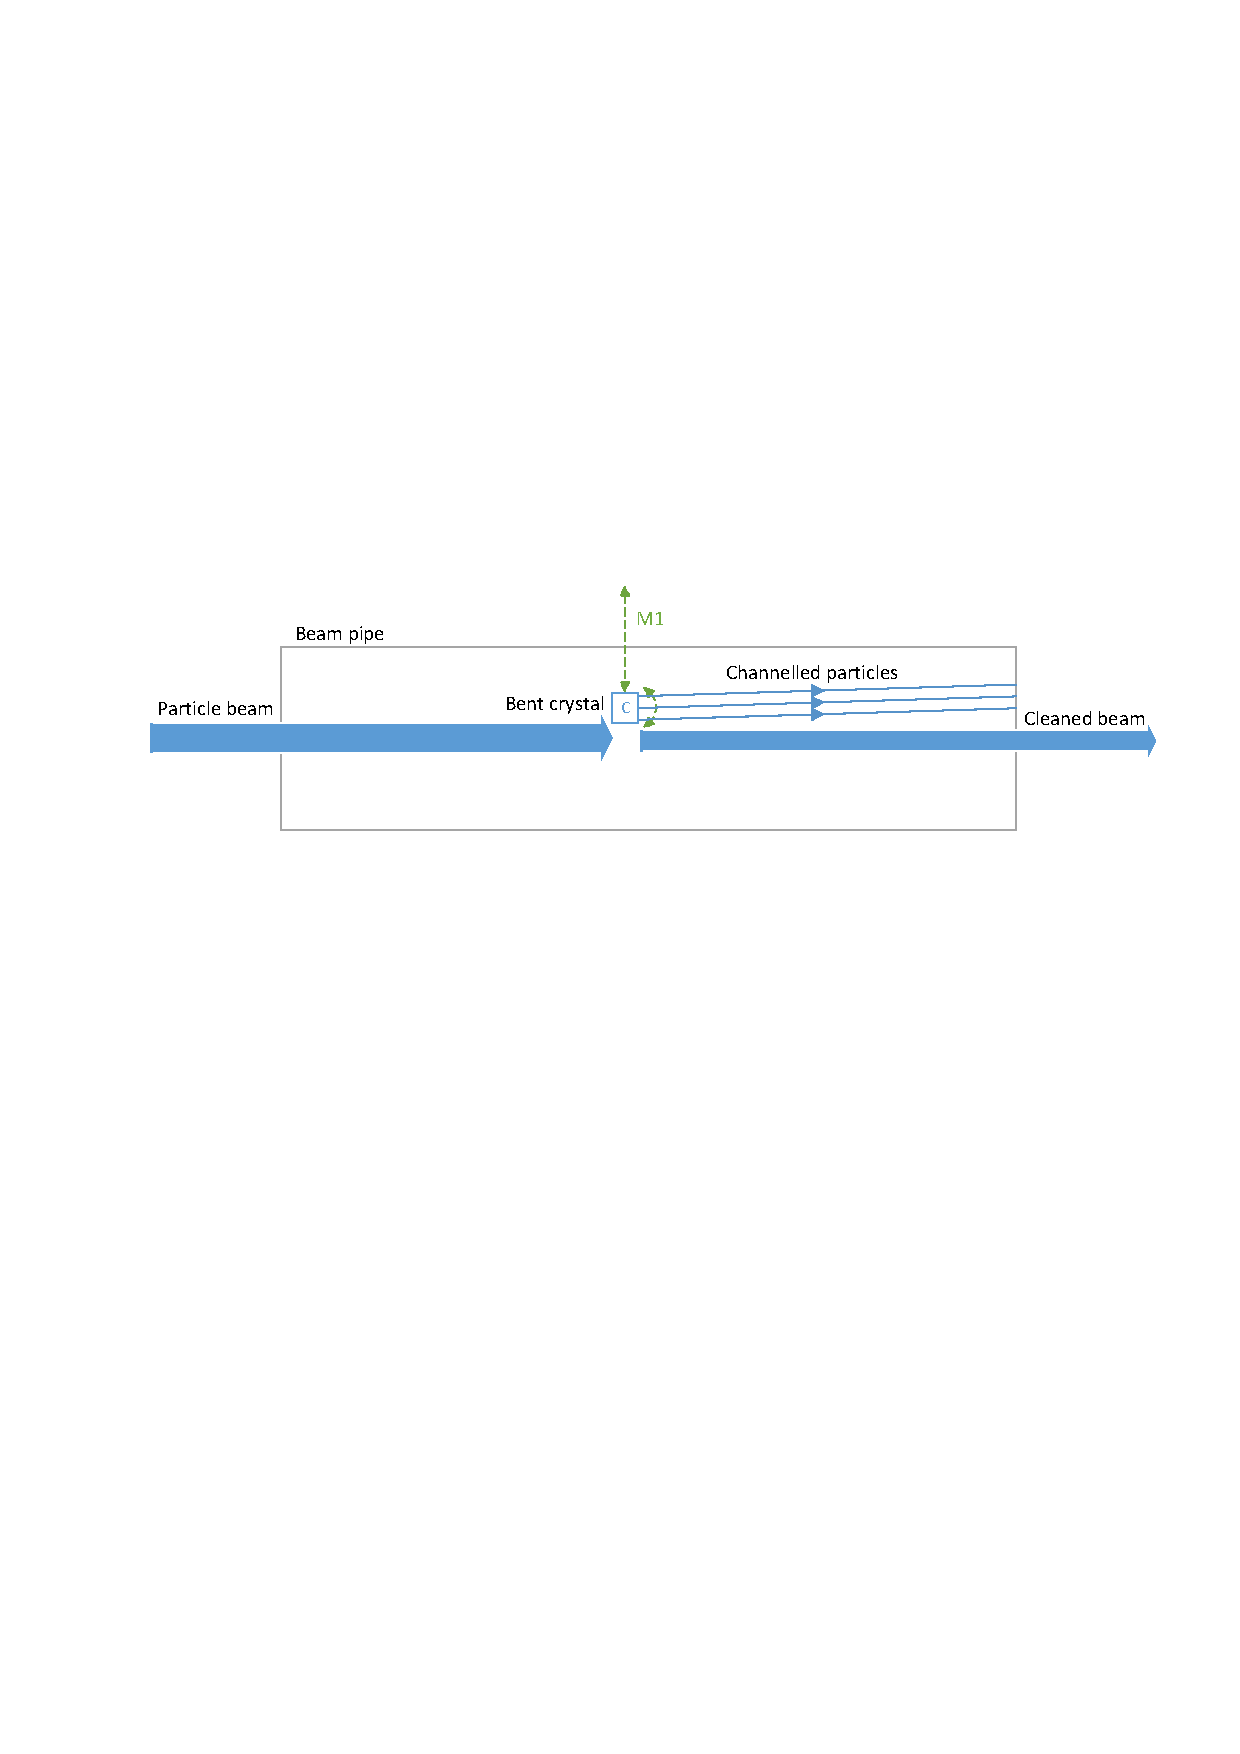
\includegraphics[width=1\textwidth, trim= 2cm 15cm 1cm 10cm, clip=true]{fig/matlab/collimation}
  \caption{\label{fig:collimation}Illustration of the crystal collimation principle as seen from above. The green dashed line represents the linear and the rotational stage movement.}
\end{figure}

The block named "C" represents the bent crystal which can be moved into the beam by the linear stage and rotated by the rotational stage that is attached to the linear axis. The crystal's linear and rotational movement are indicated in the figure as green dashed lines. During operation, physicists will drive the crystal close to the beam, enter it with an angle and rotate it slightly (in the range of \unit{1}{\milli\rad}) until the channeling effect is detected. Channeled particles (illustrated as arrowed lines in Figure~\ref{fig:collimation}) will then bend off from the beam core to be absorbed further down the beam pipe.

The collimator unit consists of a T-shape structure containing two linear and one rotational stage, as partly illustrated in Figure~\ref{fig:goniometer}.

\begin{figure}[h]
  \centering %crop: left bottom right top
  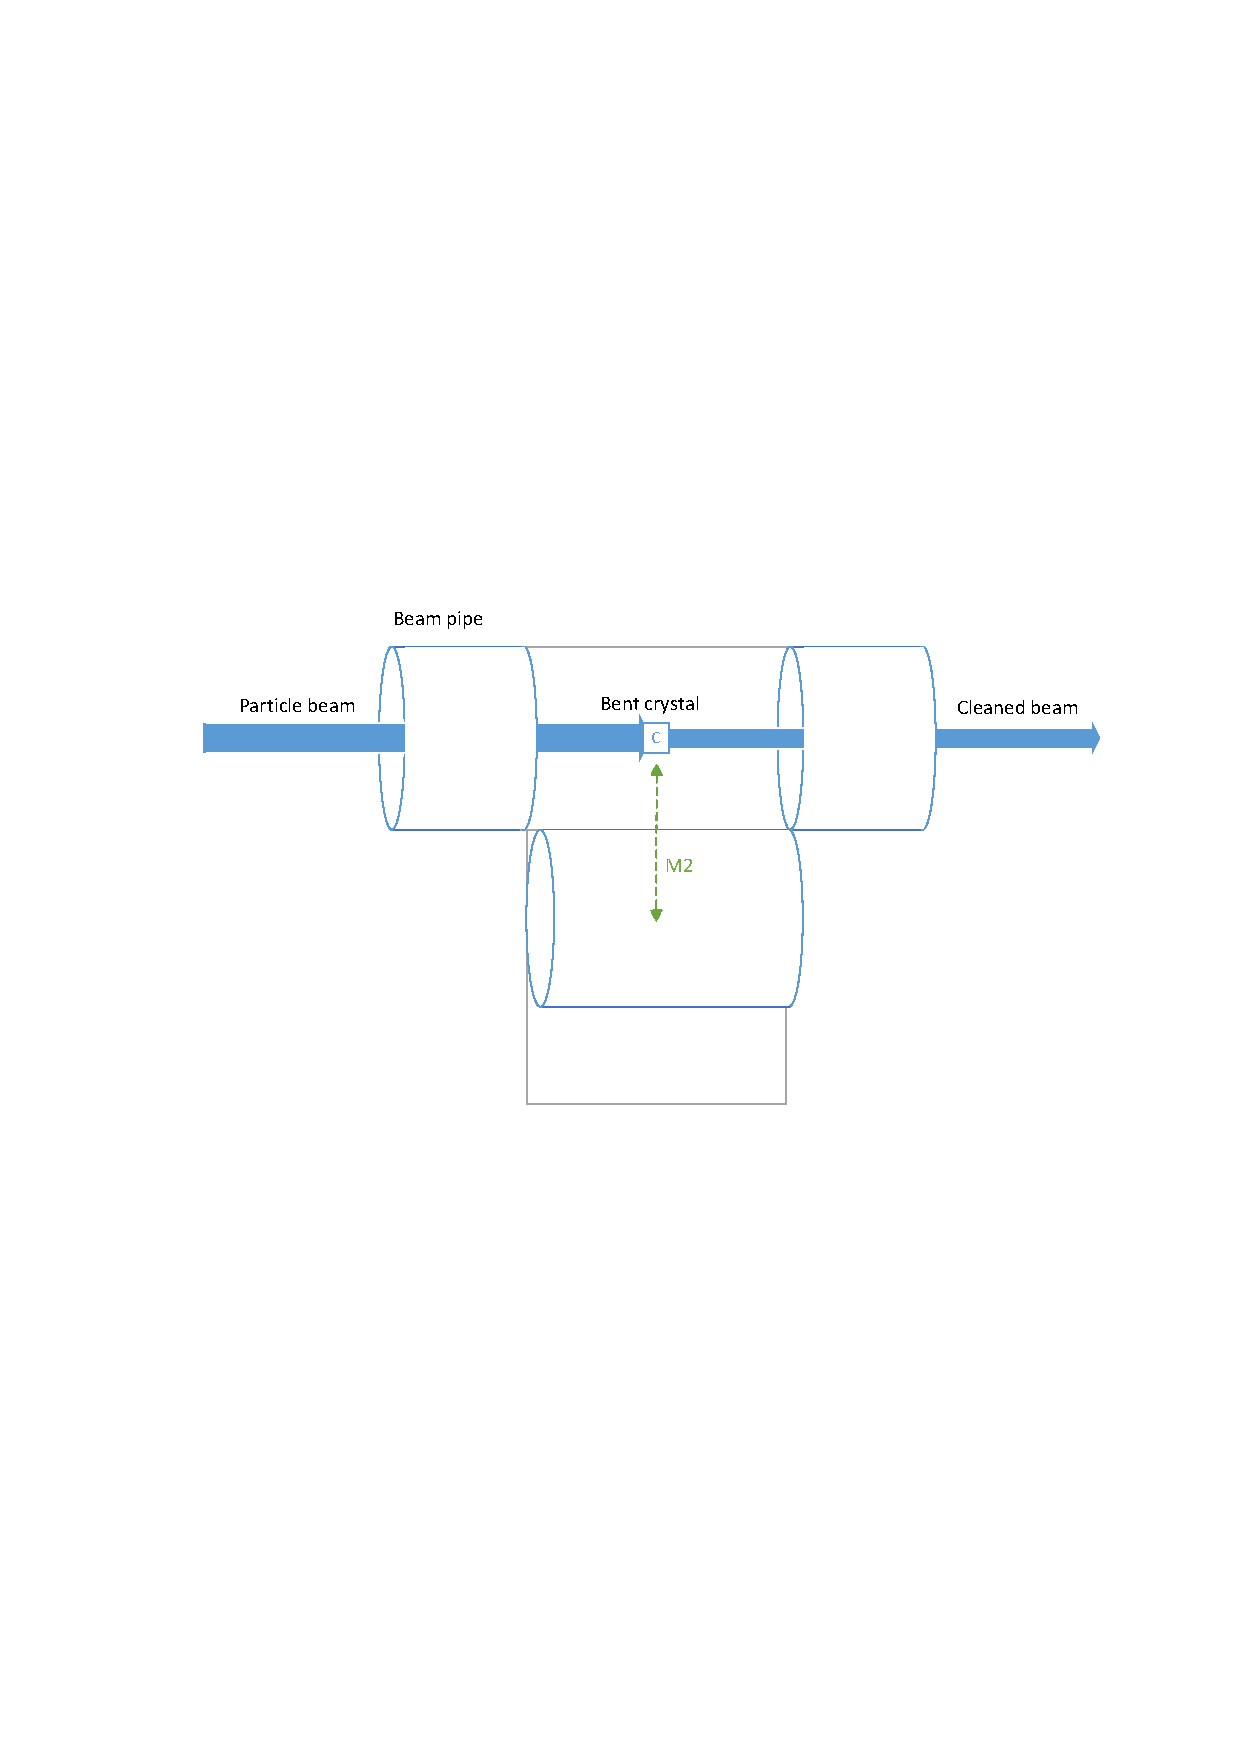
\includegraphics[width=1\textwidth, trim= 2cm 12cm 1cm 10cm, clip=true]{fig/matlab/goniometer}
  \caption{\label{fig:goniometer}Illustration of the crystal collimation principle as seen from the side. The green dashed line represents the movement of the beam pipe piece.}
\end{figure}

Each linear stage is driven by a stepping motor, labeled as \emph{M1} in Figure~\ref{fig:collimation} and \emph{M2} in Figure~\ref{fig:goniometer}, separately controlled in open-loop by an individual drive unit. The motor driving the vertical axis, \emph{M2}, is used to move a piece of beam pipe inside the T-shape, giving access to the crystal to enter and to close it when the collimation system is out of operation. This movement is illustrated in Figure~\ref{fig:goniometer} with a green dashed line.

Figure~\ref{fig:collimator} shows the new collimator. In the top view the rotational and the linear horizontal stage is indicated by labels. In this figure, the rotational stage is in its outer position. During operation it will be pushed forward by the linear axis into the beam pipe. Figure~\ref{fig:collimator-through} shows the inside of the beam pipe during movement of the beam pipe piece, the same movement that Figure~\ref{fig:goniometer} is illustrating. In Figure~\ref{fig:collimator-mirror} the crystal support has been injected into the beam pipe, note that the crystal itself is in this picture replaced by a small circular mirror.

\begin{figure}[tpb]
  \centering %crop: left bottom right top
  \subfloat[][\label{fig:collimator-side}Side view]{
  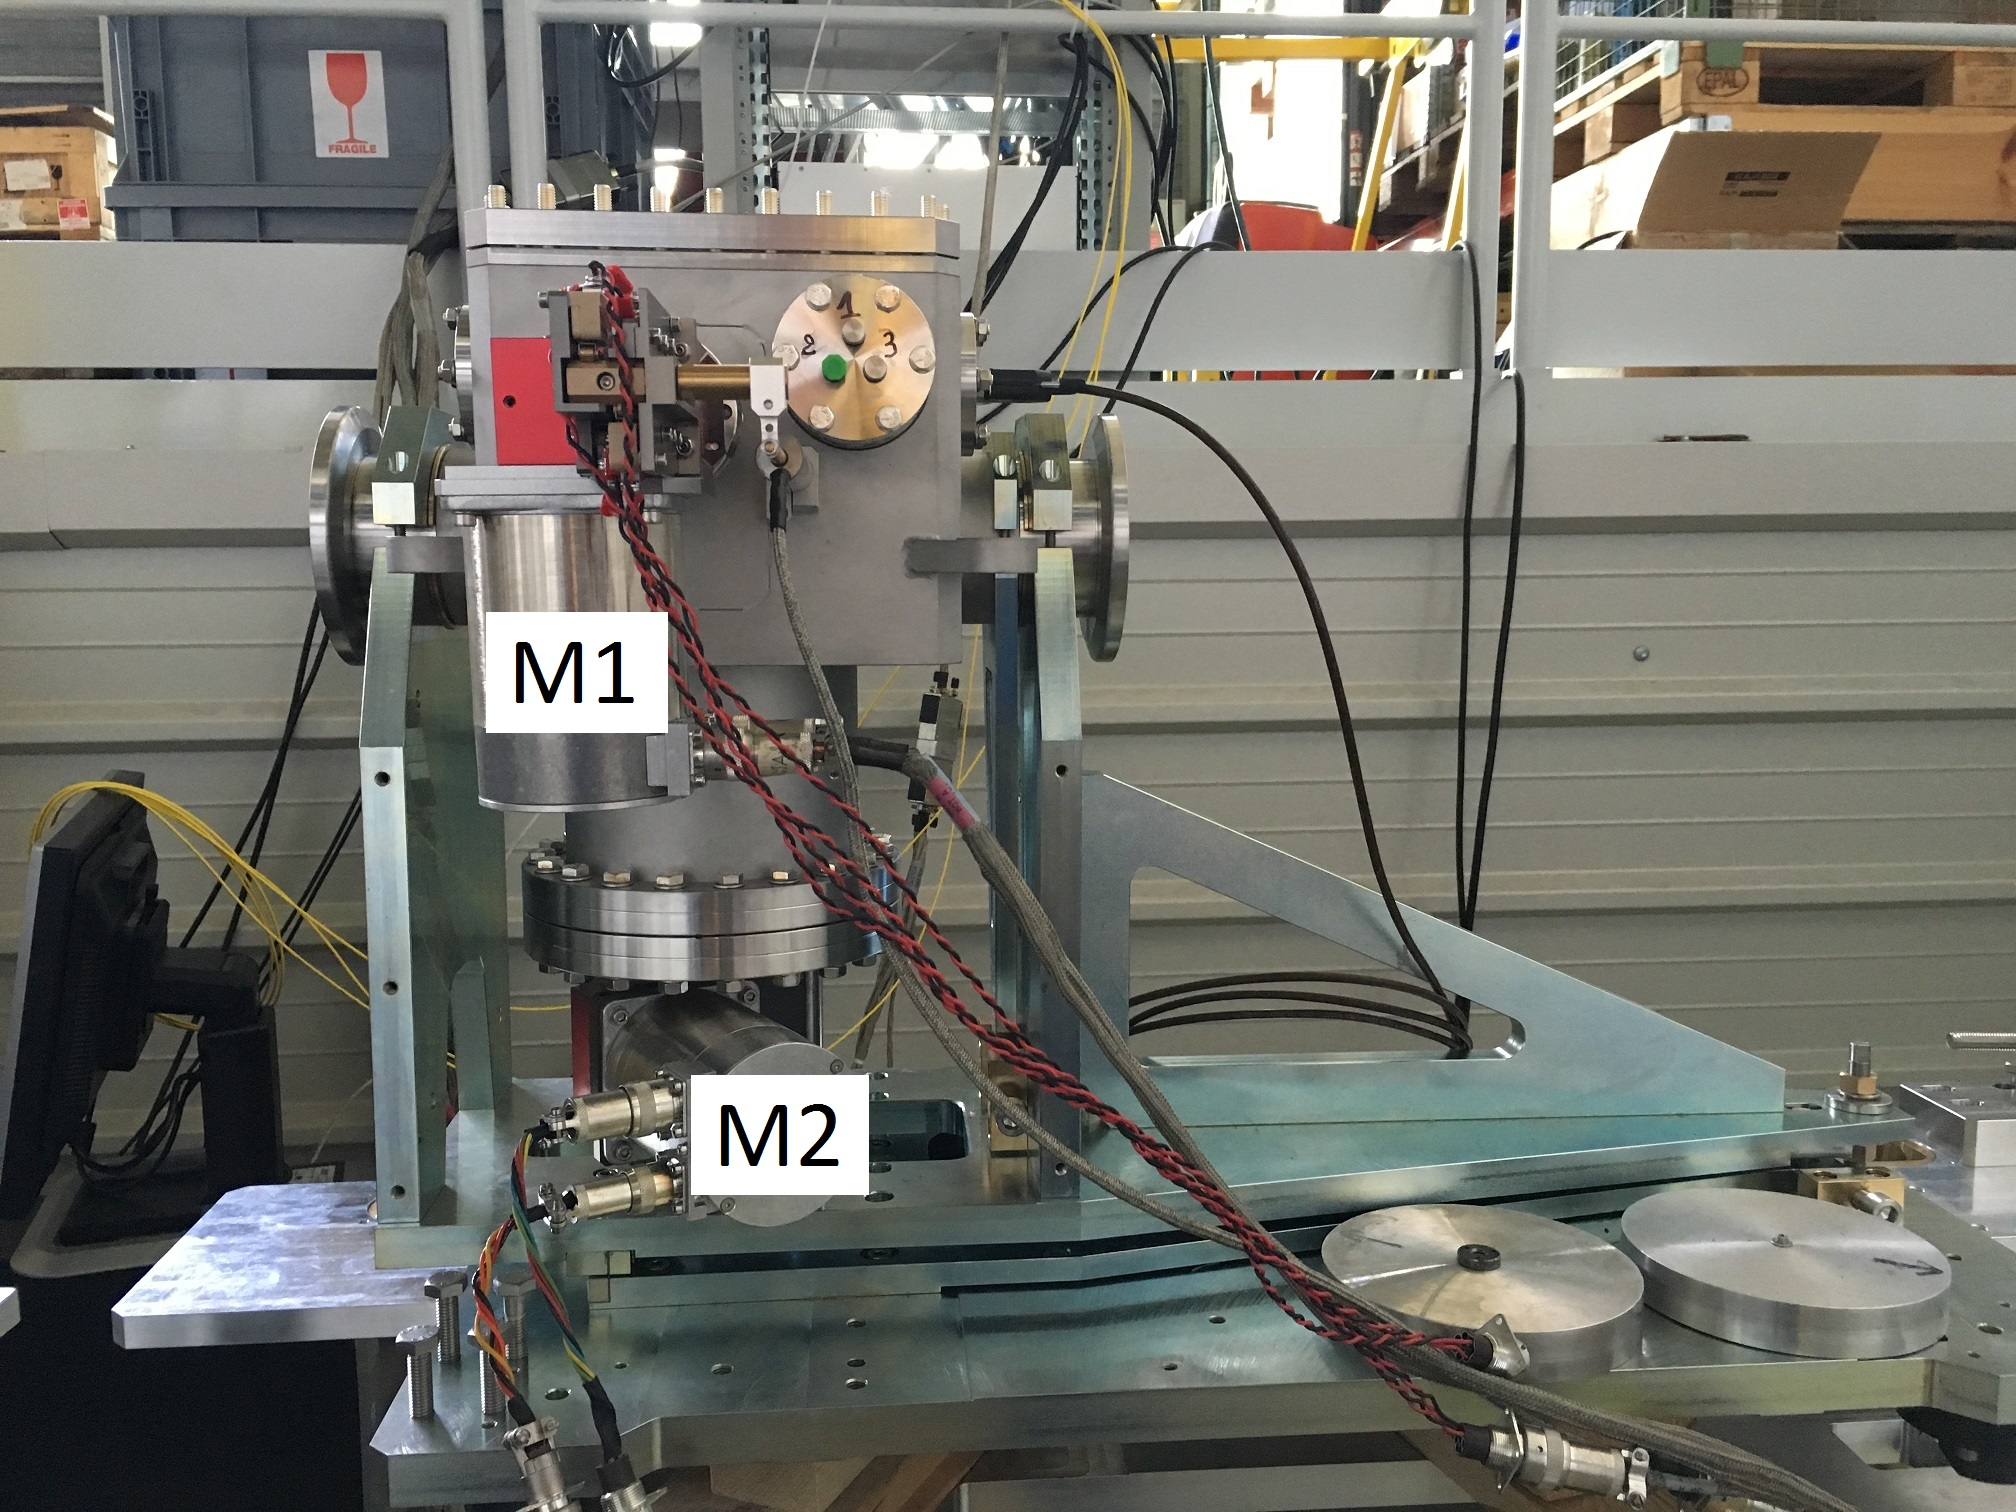
\includegraphics[width=0.5\textwidth, trim=2cm 11cm 2cm 5cm, clip=true]{fig/collimator-side}}
  \qquad
  \subfloat[][\label{fig:collimator-top}Top view]{
  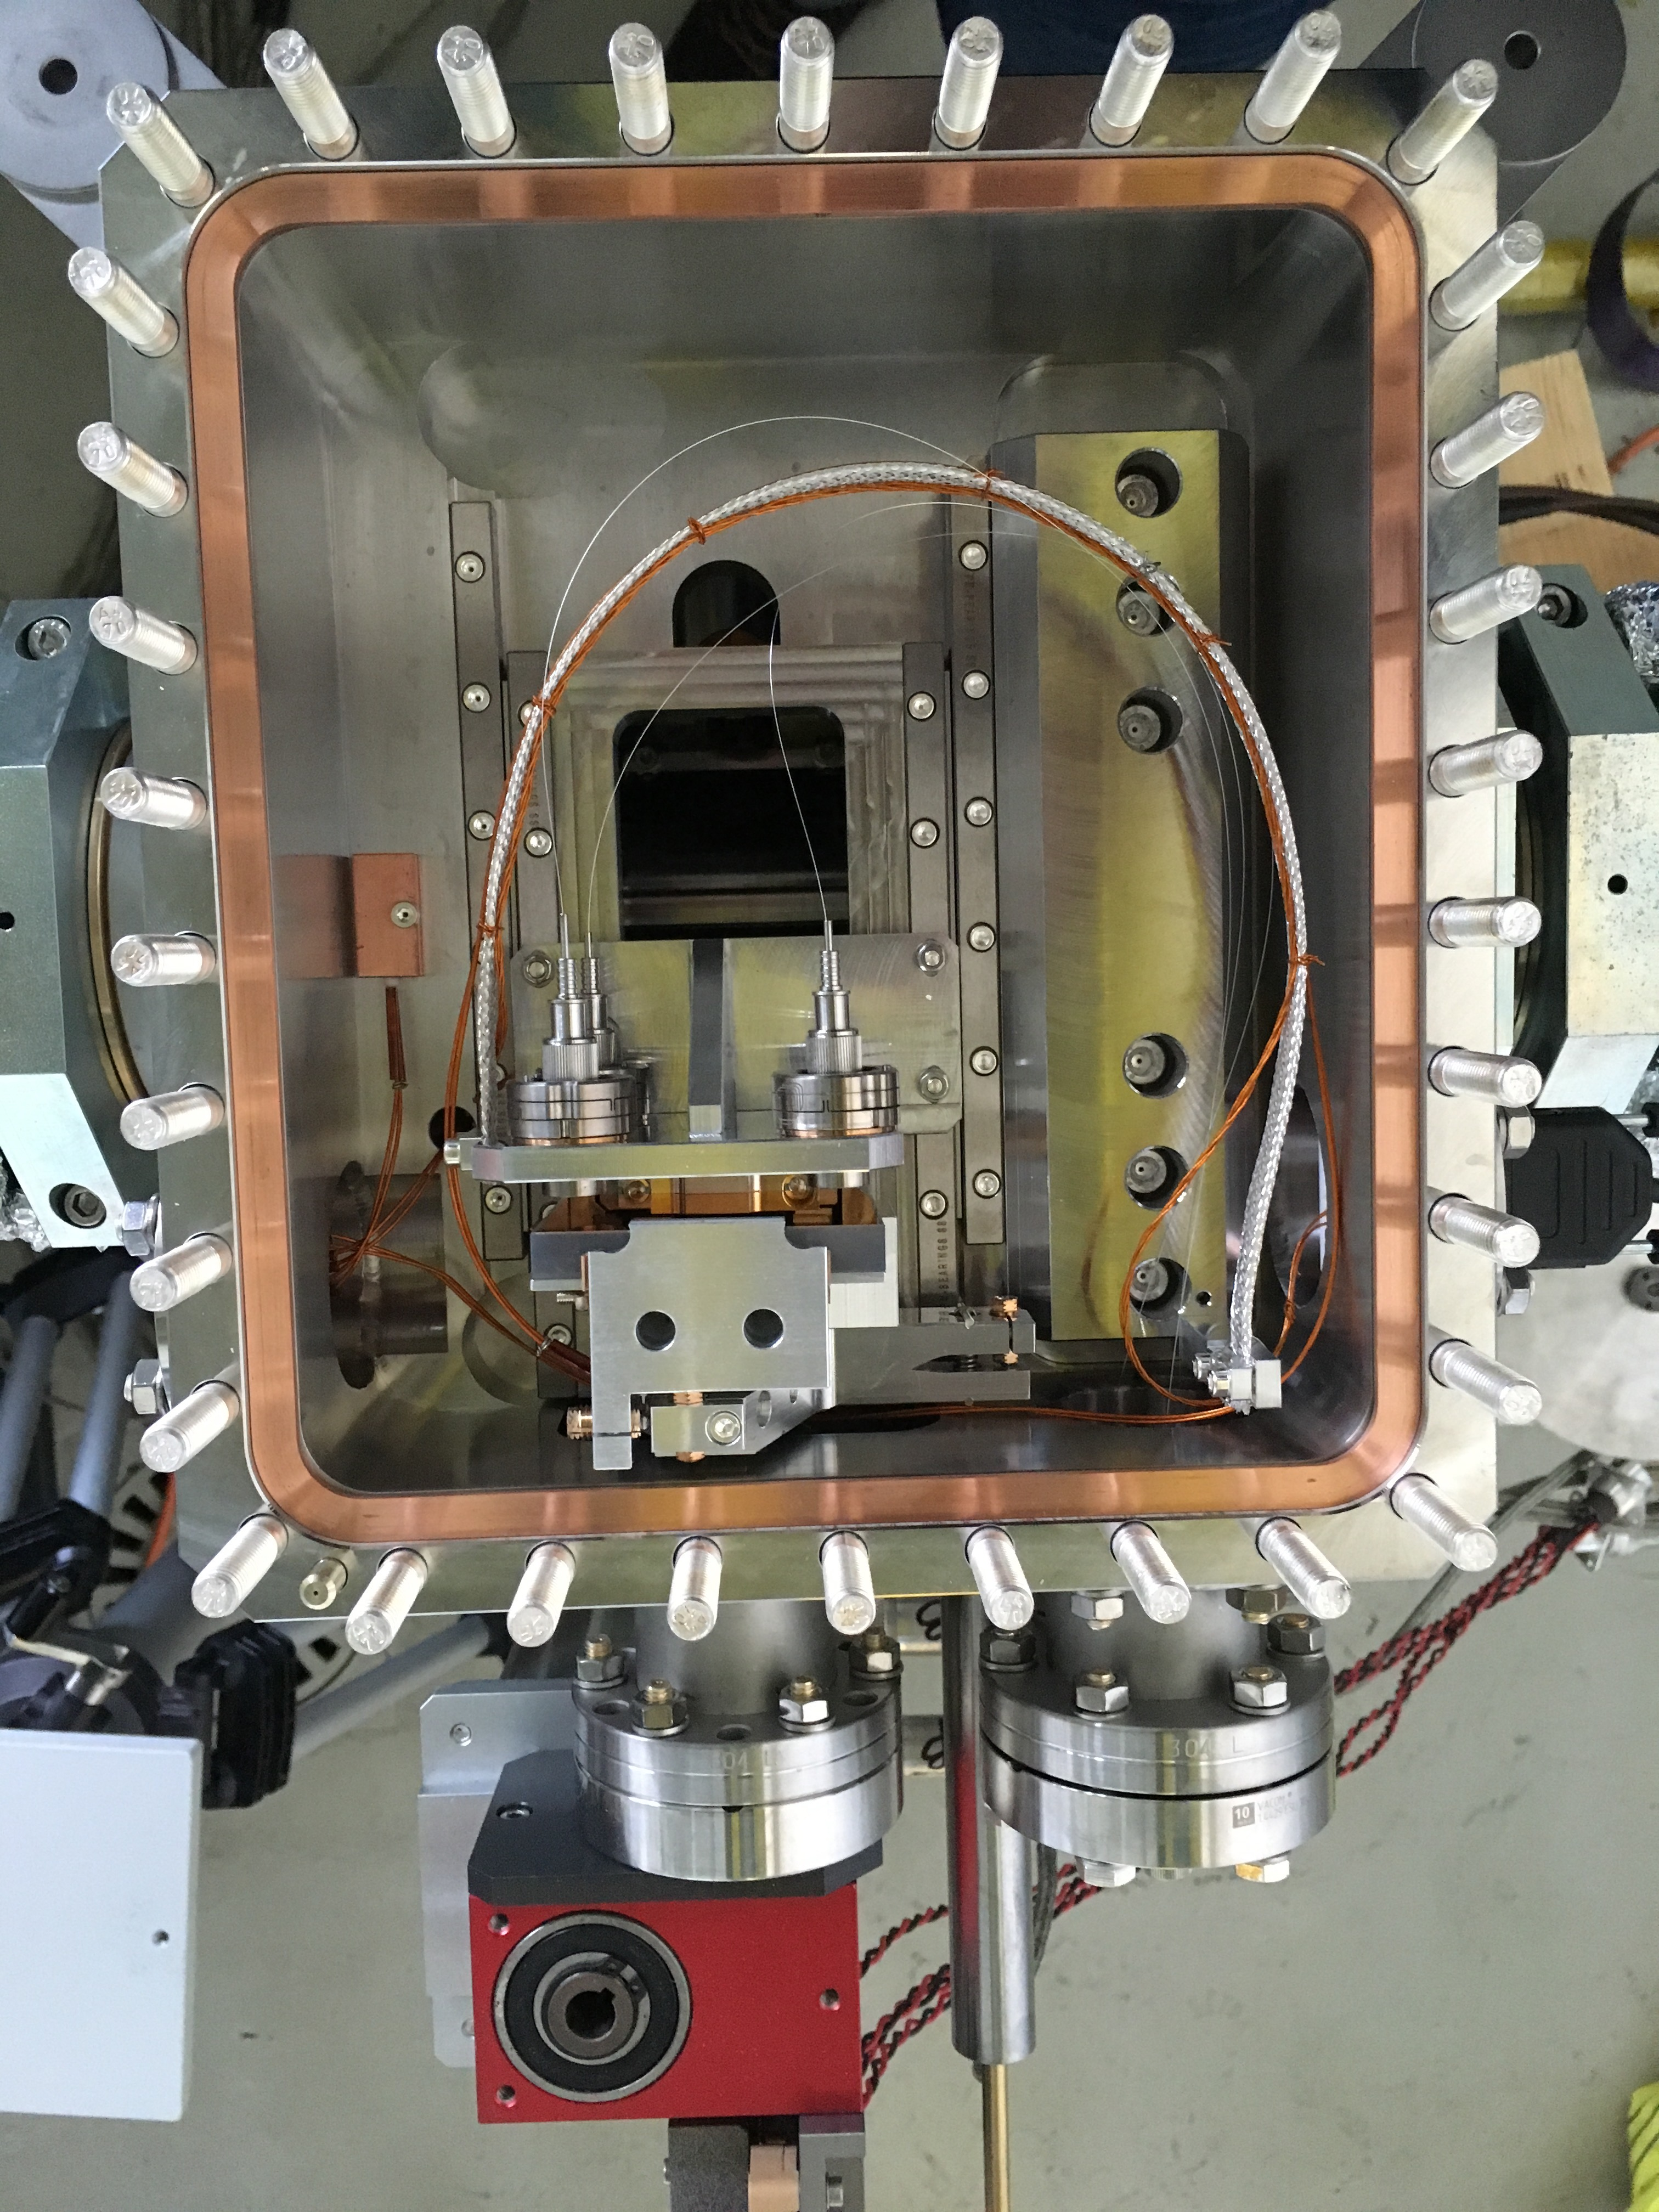
\includegraphics[width=0.42\textwidth, trim=0cm 0cm 0cm 0cm, clip=true]{fig/collimator-top}}
  \caption{\label{fig:collimator} The new collimator from the side (a) and the top (b).}
\end{figure}

\begin{figure}[tpb]
  \centering %crop: left bottom right top
  \subfloat[][\label{fig:collimator-through} Giving access]{
  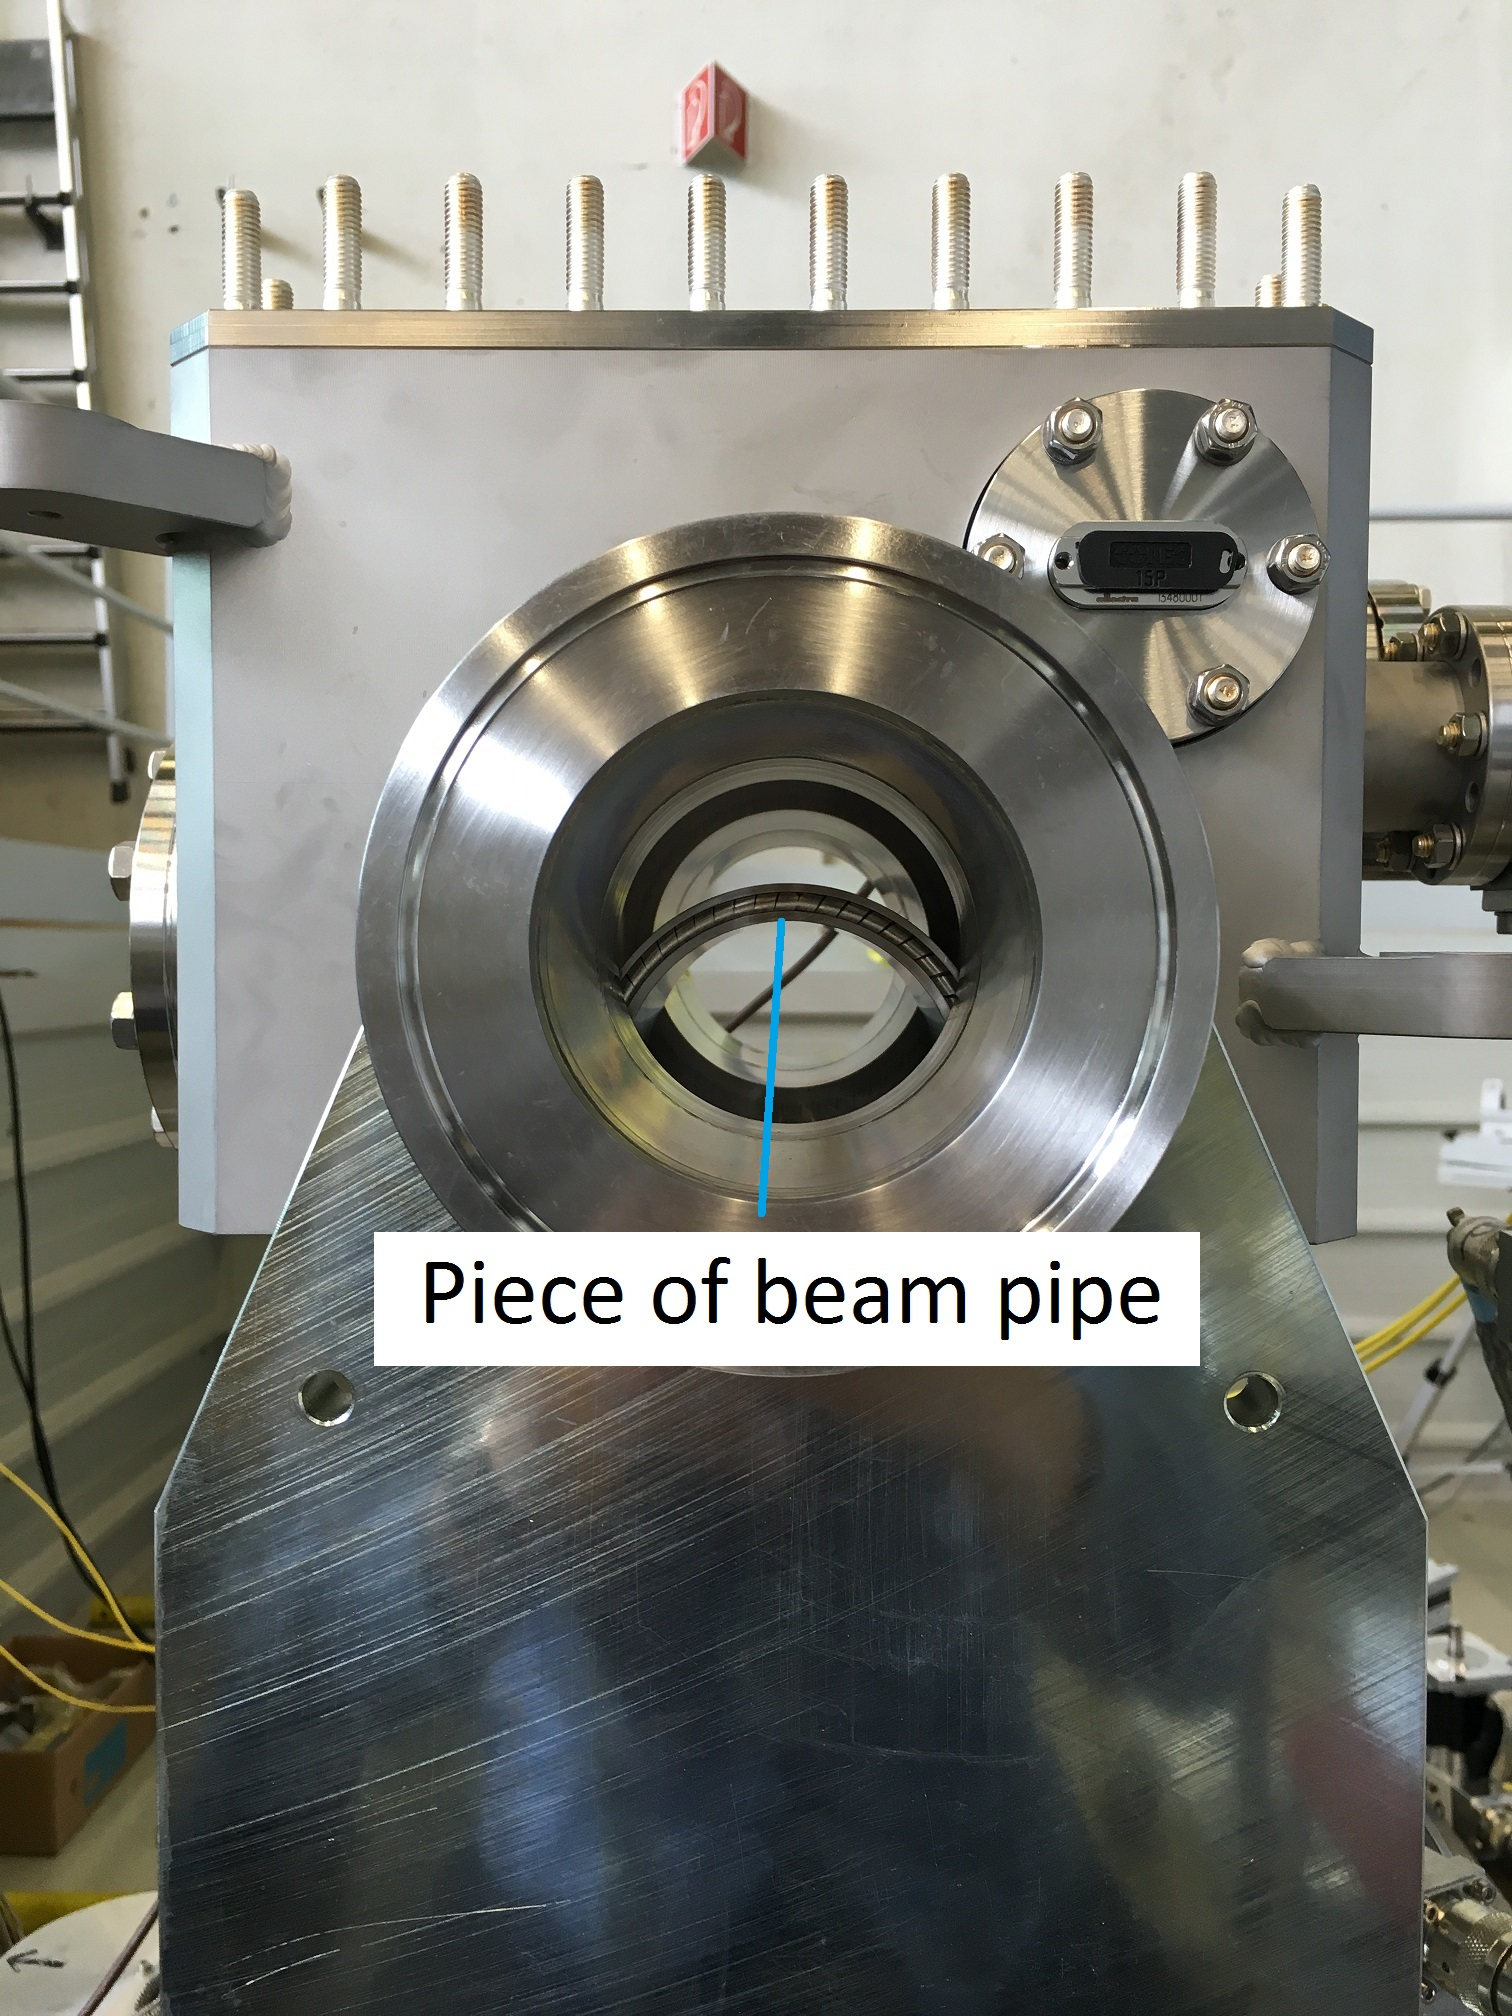
\includegraphics[width=0.42\textwidth, trim=3cm 12.8cm 2cm 5cm, clip=true]{fig/collimator-through}}
  \qquad
  \subfloat[][\label{fig:collimator-mirror} Insertion of crystal]{
  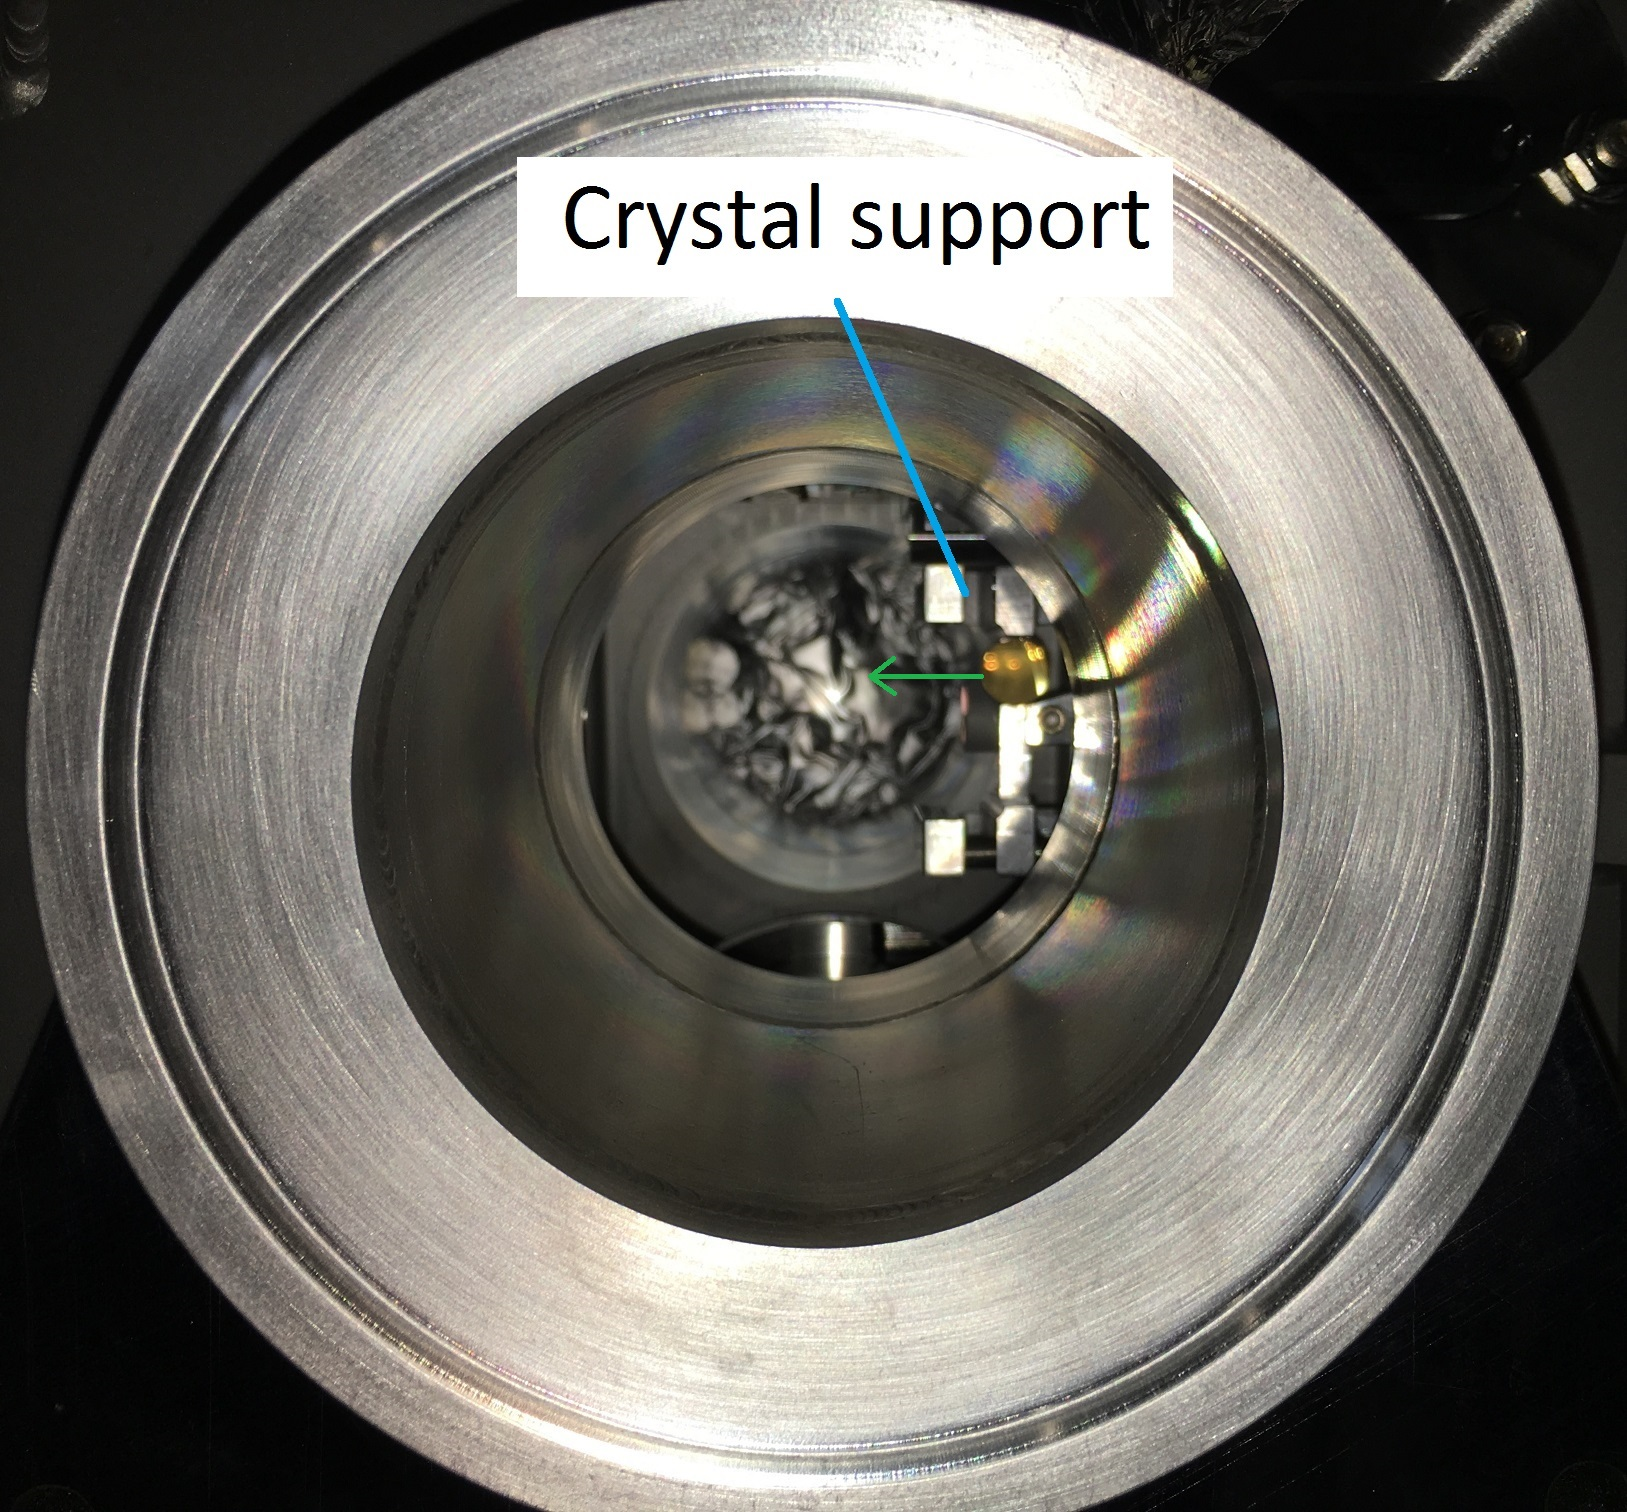
\includegraphics[width=0.5\textwidth, trim=0cm 0cm 0cm 0cm, clip=true]{fig/collimator-mirror}}
  \caption{\label{fig:collimator-t} The new collimator with the beam pipe piece half-way out (a) and the crystal inserted into the beam pipe (b).}
\end{figure}

\FloatBarrier
\section{Rotational stage}
\label{sec:rotational_stage}
The rotational stage as shown in Figure~\ref{fig:rotationalstage} is composed by a monolithic amplifying structure, a prestressed piezoelectric stack actuator and an interferometer measurement system. The flexure-hinge based structure, avoids sliding parts and thereby enhance precision by reducing the number of nonlinear effects (e.g. backlash and friction). A piezoelectric stack actuator is exploited to generate the rotational movement by interacting on a amplifying lever that applies the force on the rotational head a few millimeters from the center of rotation, marked as a red "X" in the picture. This amplifying structure gives the rotational stage a range of \unit{20}{\milli\rad} from a nominal linear range of \unit{40}{\micro\meter}.  The \abbrPEA is prestressed in order to enhance the overall stiffness as well as keeping the stack in place (the stack is non-glued to be sufficient in a radioactive area). This combination leads to a clear resonant structure, due to the characteristics of the \abbrPEA and the flexible structure, demanding a properly designed controller.

\begin{figure}[h!]
  \centering
  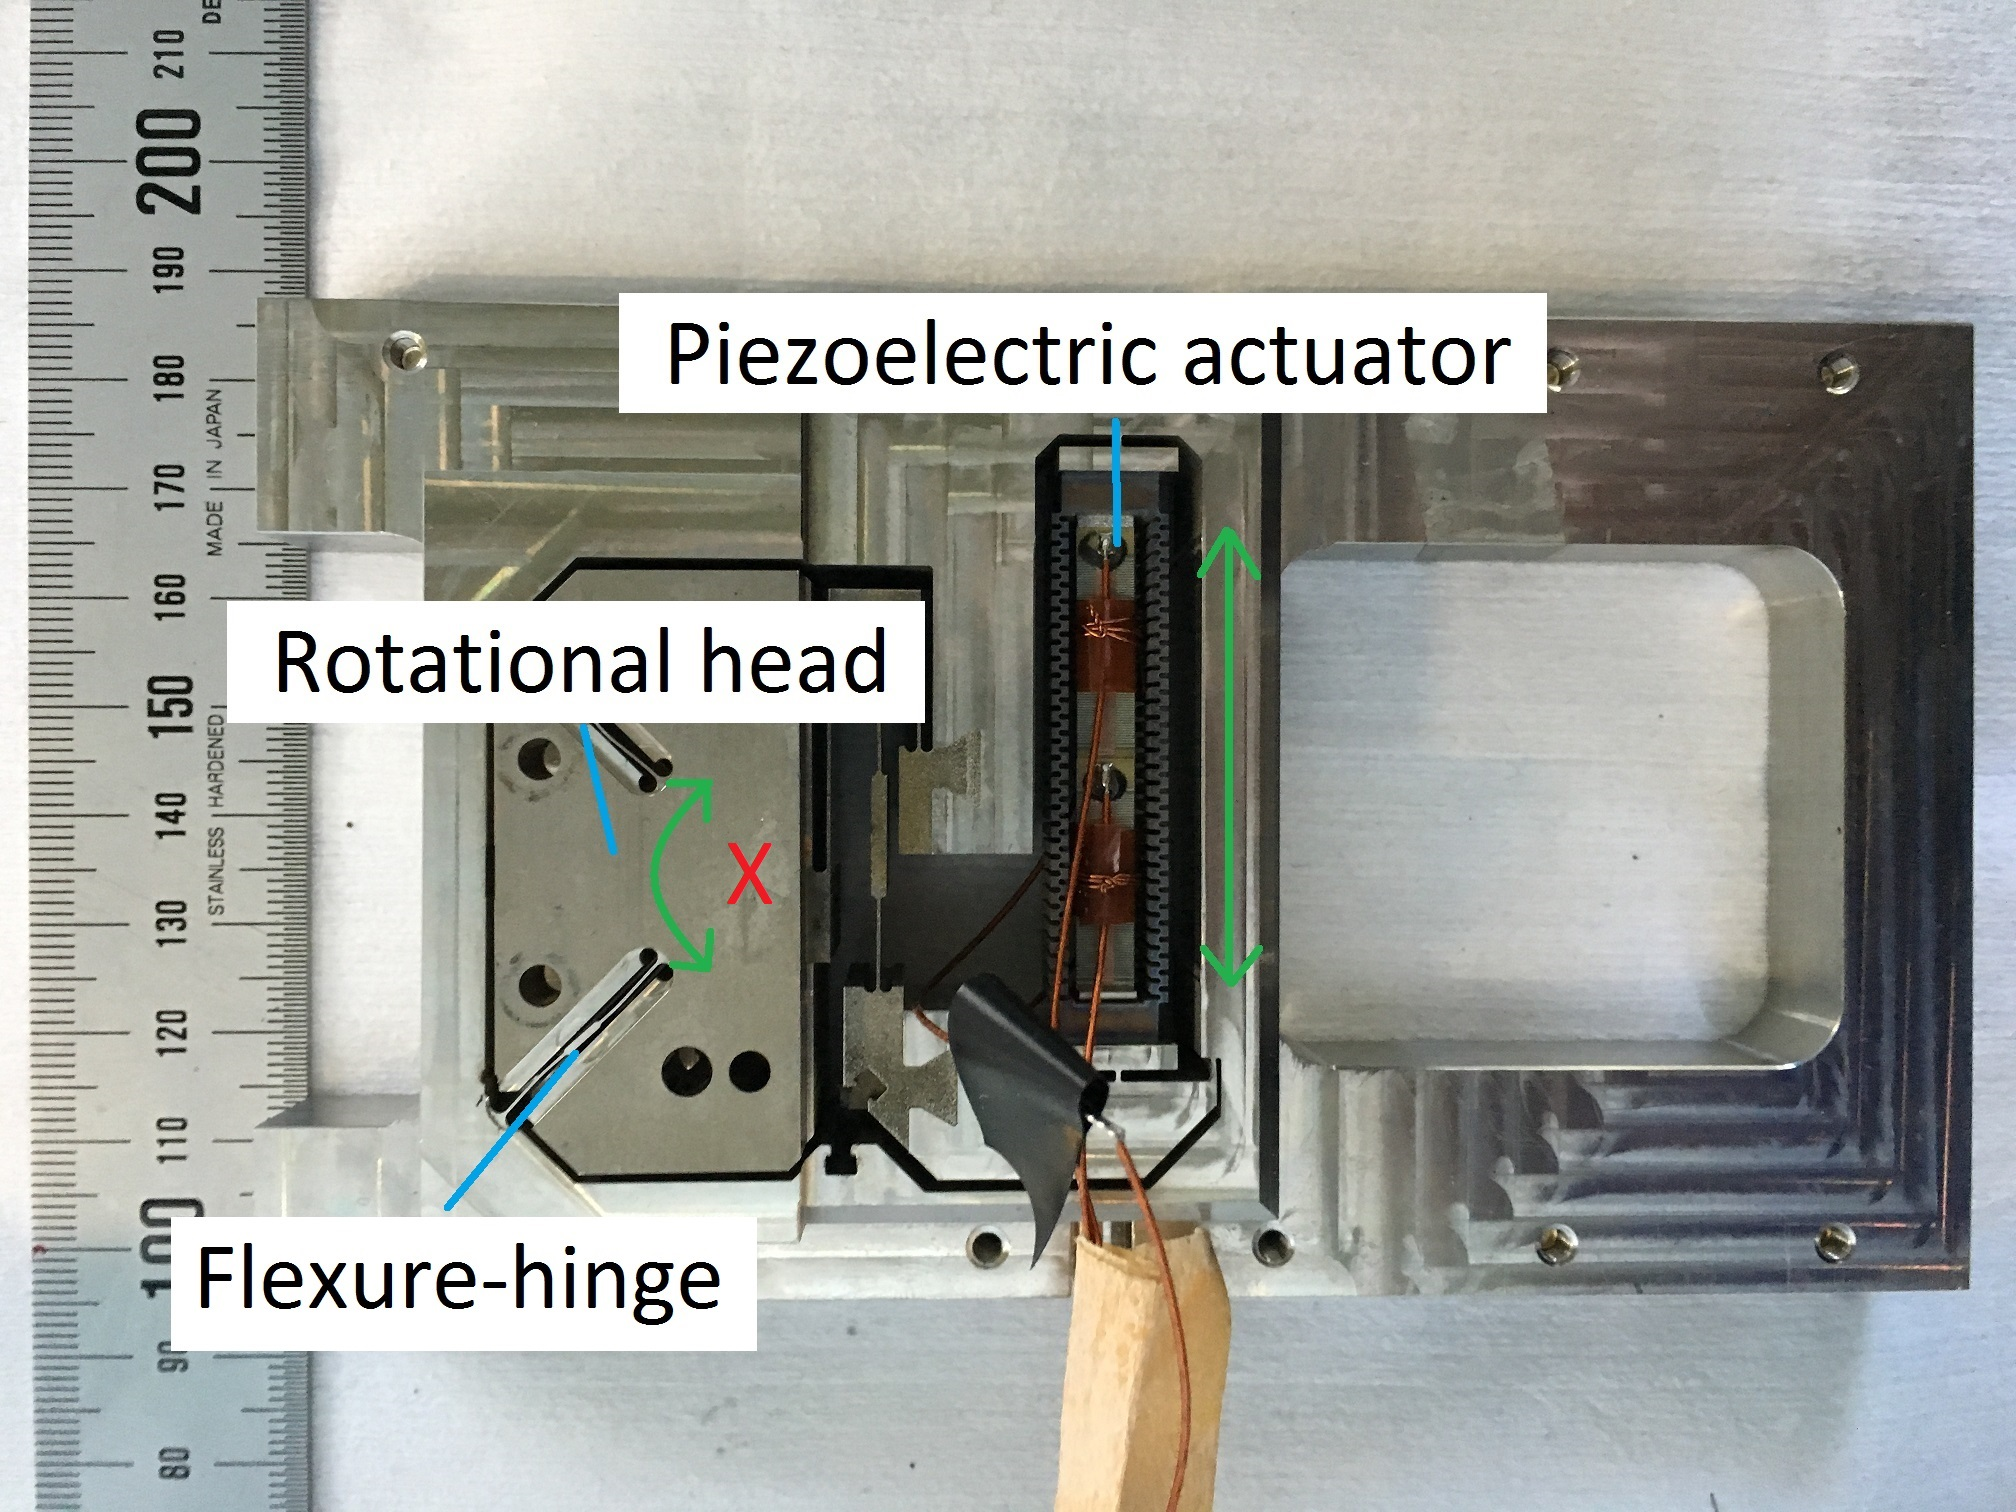
\includegraphics[width=0.7\textwidth]{fig/rotational-stage.jpg}
  \caption{\label{fig:rotationalstage} Piezo-actuated rotational stage used in the new collimator.}
\end{figure}

For the measurement system, three interferometric heads are placed on top of the rotational stage as seen Figure~\ref{fig:rotationalstage-side}, pointing towards a mirror that is attached to the crystal support and to the rotational head, perpendicular to the plane of rotation. The setup allows for measurements of both the yaw and roll angle (the coordinate system is defined with respect to the beam), but only the yaw angle is used in the feedback to the rotational stage control loop. Note that the crystal is mounted below the rotational head and that only the top of the crystal support is shown in the picture.

\begin{figure}[h!]
  \centering
  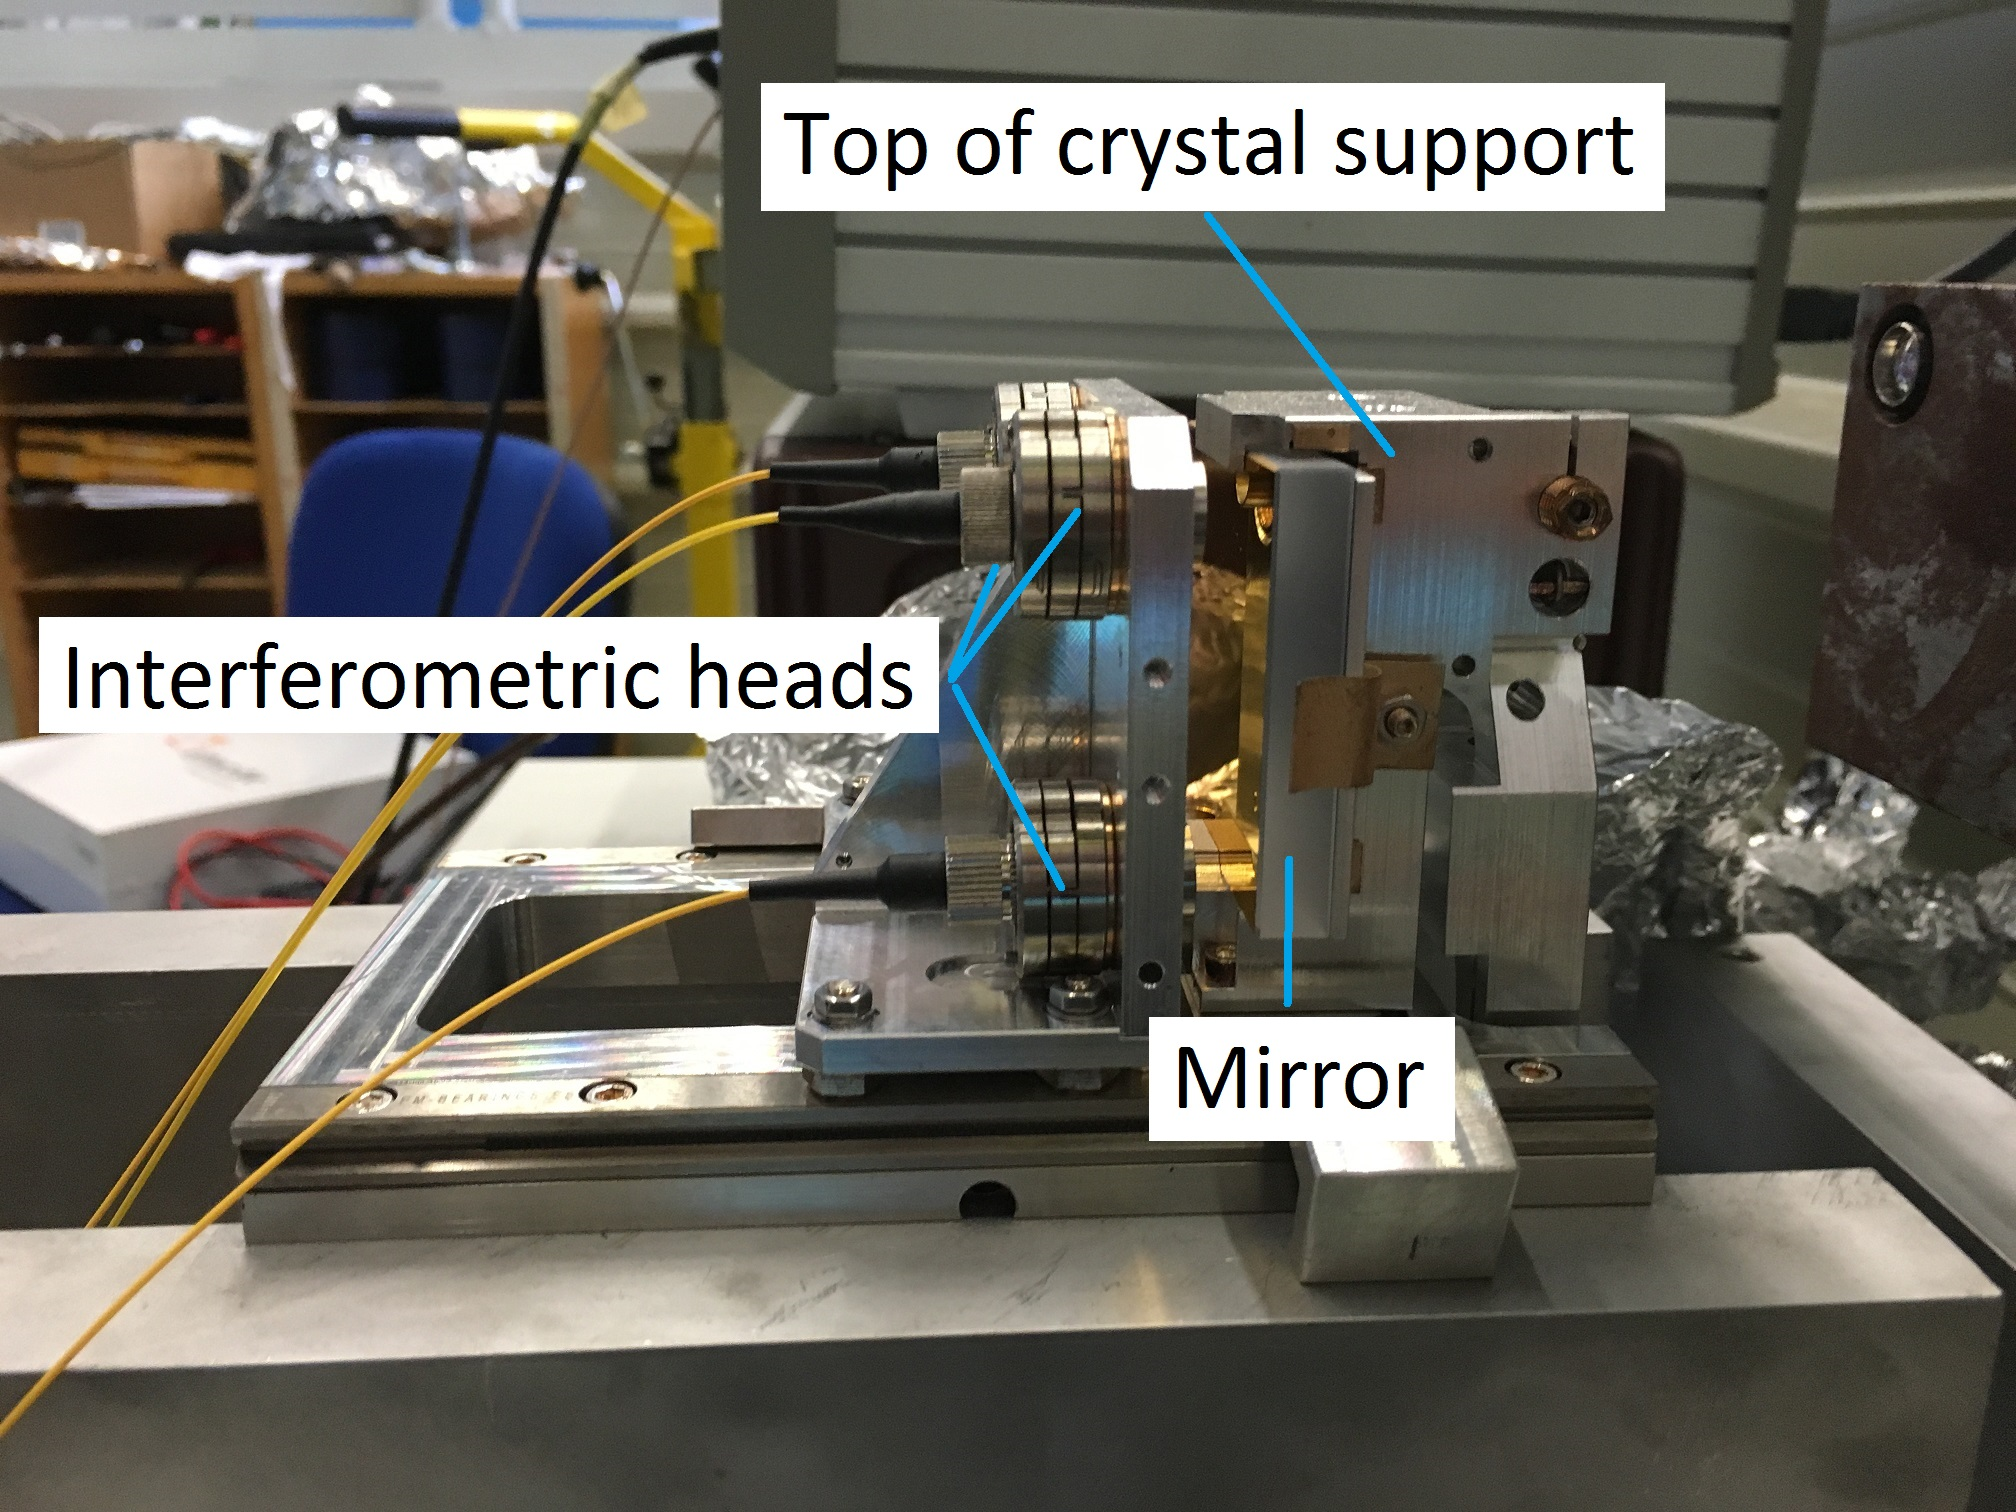
\includegraphics[width=0.7\textwidth]{fig/rotational-stage-interferometer.jpg}
  \caption{\label{fig:rotationalstage-side} Rotational stage with the crystal support and the interferometric system mounted on top.}
\end{figure}

\section{Piezoelectric Stack Actuators}
The rotational stage uses a linear piezoelectric stack actuator to create the movement. It provides a displacement range from 0 to \unit{30}{\micro\meter}, corresponding to -20 and +150V, respectively. The actuators are made of many thin, stacked electro-active ceramic disks, electrically connected in parallel. This construction allows for a high stiffness actuator that still can exhibit long displacement ranges \cite{Piezo:2008}.

\subsection{Hysteresis Effect}
The hysteresis effect is a nonlinear effect that is present during the operation of piezoelectric actuators. It occurs when the driving direction is reversed and origins from the polarization and the molecular effects in the piezo-ceramic. It depends on the amplitude of the applied voltage but also on the frequency of the input signal \cite{Qingson:2016}. Figure~\ref{fig:hysteresis} illustrates the hysteresis effect. One can see how the same voltage, e.g. 60V, corresponds to an angular position of \unit{5.2}{\micro\rad} in one direction and to \unit{7.2}{\micro\rad} in the opposite direction.

\subsection{Creep Effect}
The creep effect is another nonlinear effect that is present during the operation of piezoelectric actuators. The effect is a slow elongation or contraction of the actuator displacement over time with a constant driving signal and is caused by thermal effects in the piezo-ceramics. Figure~\ref{fig:creep} illustrates the creep effect. One can see how the rotational stage slightly drifts off from the reference after the applied negative step, increasing the tracking error over time.

\begin{figure}[h!]
  \centering %crop: left bottom right top
  \subfloat[][\label{fig:hysteresis} Hysteresis loop]{
  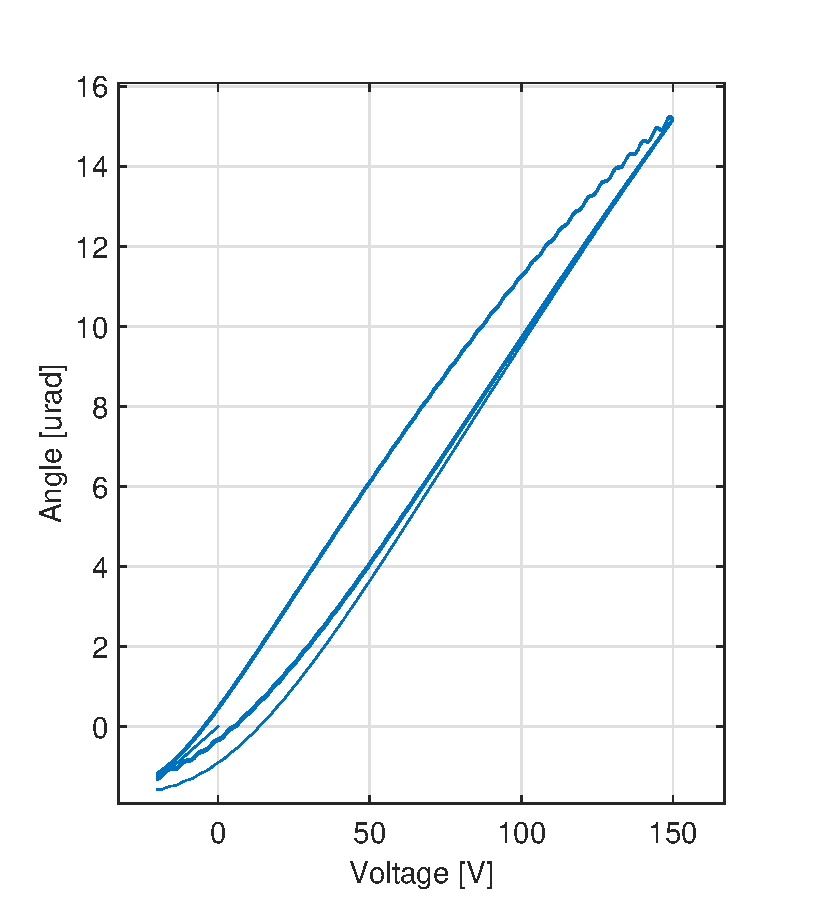
\includegraphics[width=0.46\textwidth, trim=0cm 0cm 1cm 0cm, clip=true]{fig/matlab/hysteresis.eps}}
  \qquad
  \subfloat[][\label{fig:creep} Creep effect]{
  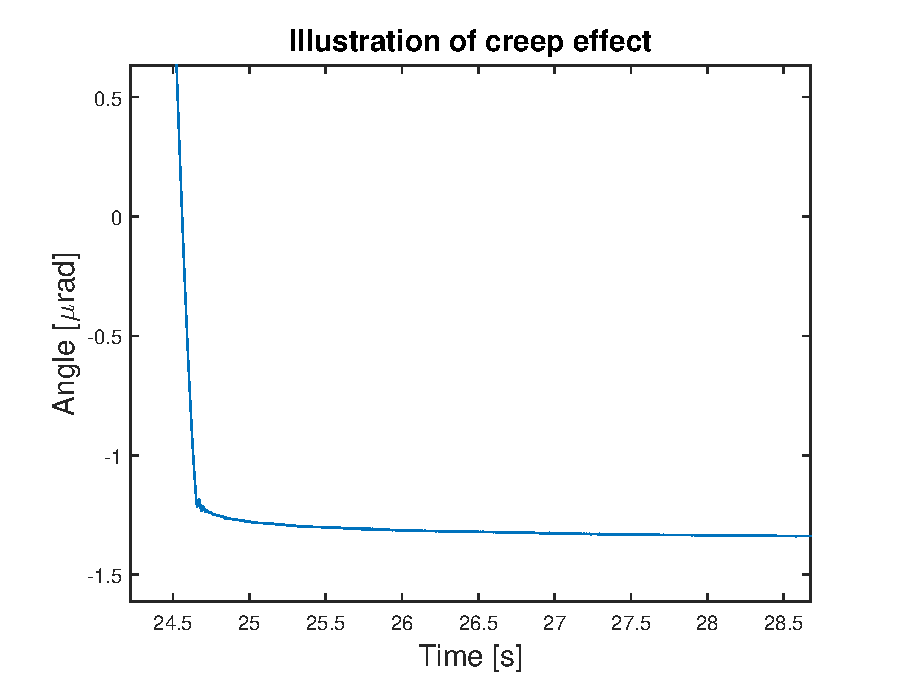
\includegraphics[width=0.46\textwidth, trim=0cm 0cm 1cm 0cm, clip=true]{fig/matlab/creep.eps}}
  \caption{\label{fig:effects} Illustration of the hysteresis effect (a) and creep effect (b). Note that the creep effect can last up to 10-15 minutes even if the plot only shows the development over 4 seconds.}
\end{figure}

The creep effect is in this project (and many others) efficiently suppressed by the feedback controller requiring no precise modeling and cancellation technique.

\section{Rotational Stage Modeling}
The piezo-actuated rotational stage is modeled by a Hammerstein structure, adopted by the authors in \cite{ButcherController:2015}, allowing them in principal, to decouple the nonlinear hysteresis from the linear system dynamics. The employed Hammerstein structure is depicted in Figure~\ref{fig:hammerstein} and consists of a \emph{Static Hysteresis} (rate independent) model and a \emph{Linear Dynamics} model. {\abbrPEA}s are known to show hysteretic behavior with a nonlocal memory (the current output does not only depend on the current input voltage but also on its history) as described in \cite{ButcherIdentification:2015}. This behavior is modeled by a generalized Maxwell-slip compensation model, described in \ref{sec:maxwell}. The extracted linear dynamics is identified using the described procedure in \ref{sec:linsys}

\begin{figure}[h]
  \centering %crop: left bottom right top
  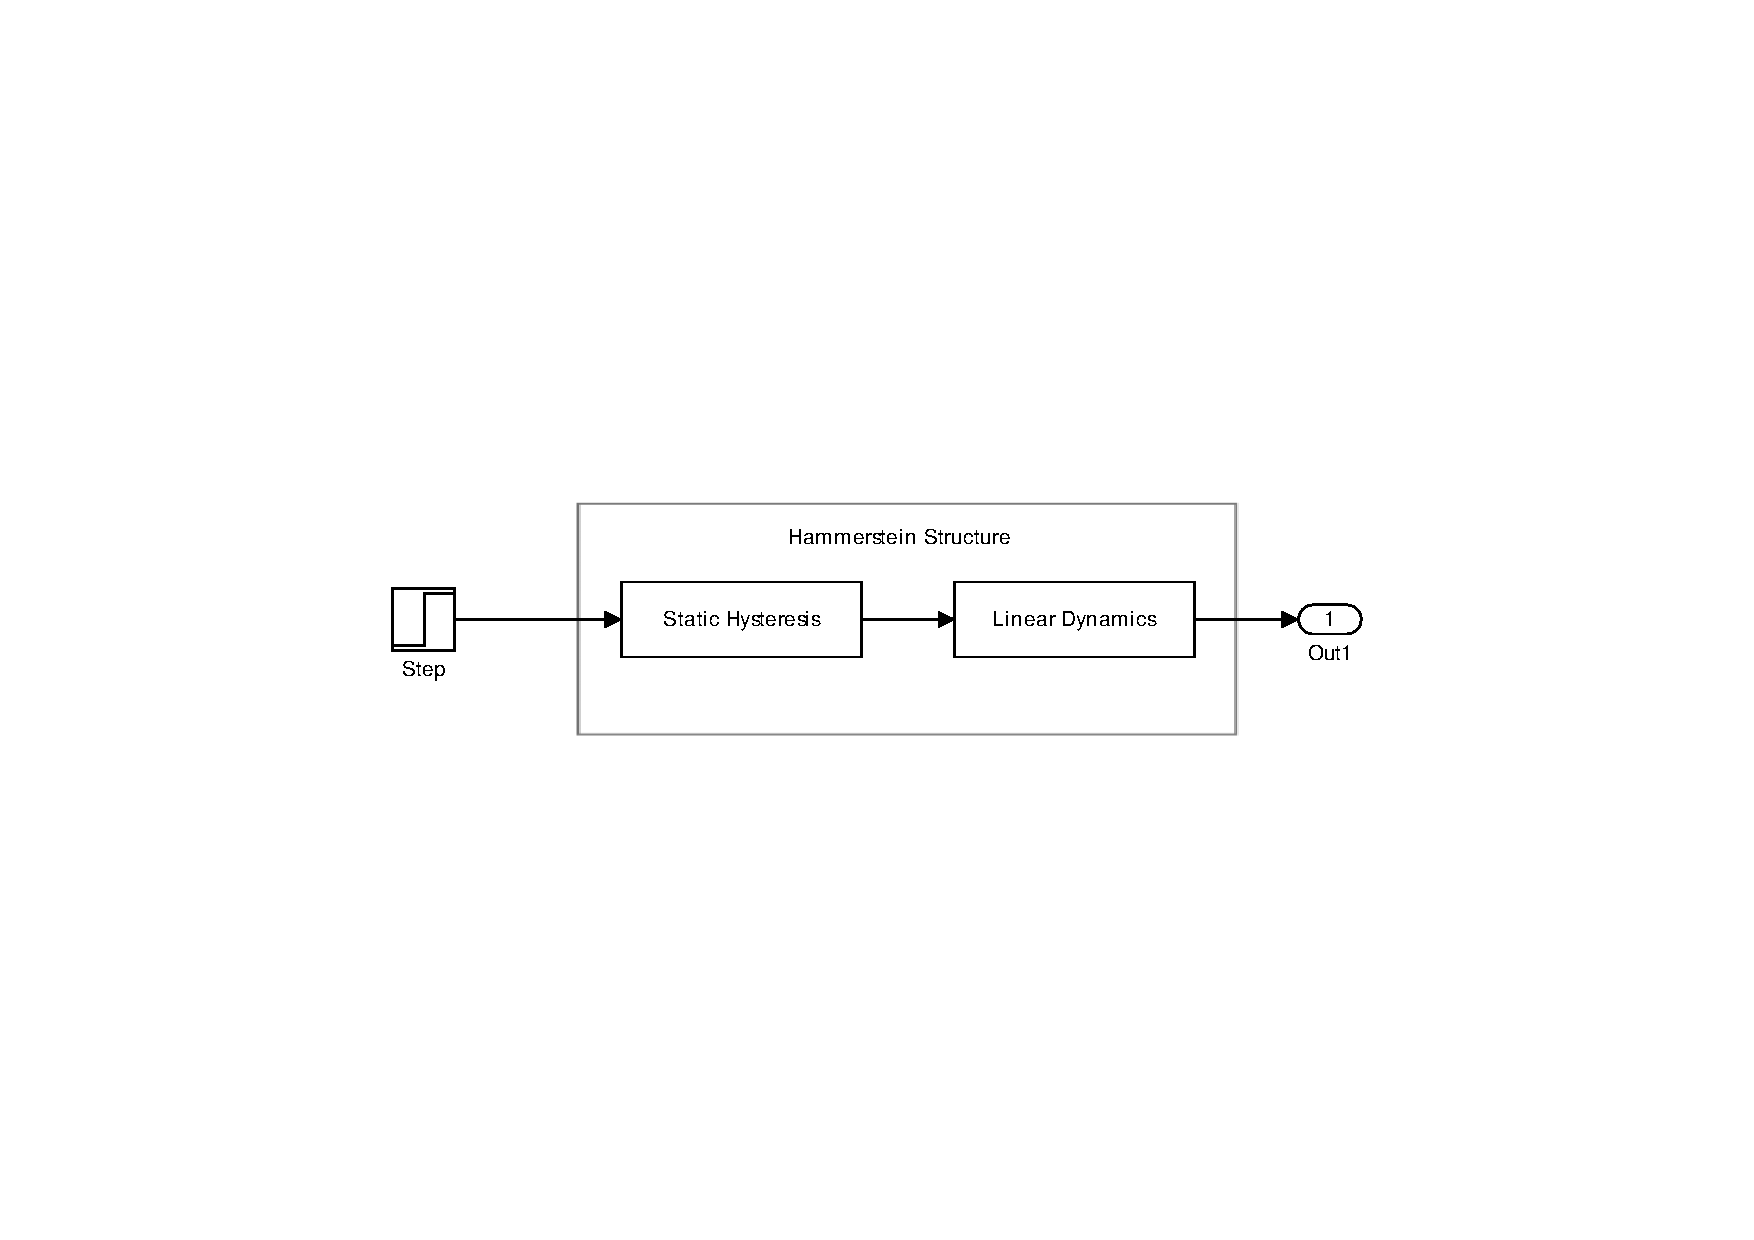
\includegraphics[width=0.7\textwidth, trim=8cm 8cm 7.73cm 8cm, clip=true]{fig/matlab/hammerstein}
  \caption{\label{fig:hammerstein}Block diagram of a Hammerstein structure, consisting of two blocks in series, modeling the static hysteresis and the linear dynamics, respectively.}
\end{figure}

\subsection{Maxwell-slip Model}
\label{sec:maxwell}
A generalized Maxwell-slip is used to model the hysteresis effect. It uses a parallel $n^{th}$ order elasto-slide element system with a friction force acting on each element, to create a nonlinear model. An elasto-slide element consist of a massless spring connected in series with a massless block that is subject to Coulomb friction. The inverse hysteresis model is summarized in the following equations and described more thoroughly in \citep{Ru:2016},

\begin{equation}
  \label{eq:maxwell_slip}
  F_i =
  \begin{cases}
    k_i(x - x_{bi}) & \quad \text{if }  k_i|x - x_{bi}| < f_i\\
    f_isgn(\dot{x}) \text{ and } x_{bi} = x - \frac{f_i}{k_i}sgn(\dot{x})  & \quad \text{else}\\
  \end{cases}
\end{equation}

\begin{equation}
  \label{eq:maxwell_sum}
  F = \displaystyle\sum_{i=1}^{n} F_i
\end{equation}

where $F_i$ is the output force, $k_i$ the spring constant, $f_i$ the break-away force and $x_b$ is the block position where $i=1 \hdots n$. In terms of the rotational stage $F_i$ represents the applied voltage, $x$ the input (rotational) displacement, $x_b$ angular position and $k_i, f_i$ are unknown parameters
The model parameters have been estimated by fitting the model to the major hysteresis loop, obtained by acquiring data from the system with a 0.5 Hz input driving signal as described in \citep{ButcherIdentification:2015,ButcherController:2015}. The identified set of parameters is presented in Table~\ref{tab:maxwell} where $n=10$. The model fit of the hysteresis model, which uses the same set of parameters as the inverse hysteresis model, is shown Figure~\ref{fig:maxwell}.

\begin{figure}[h]
  \centering
  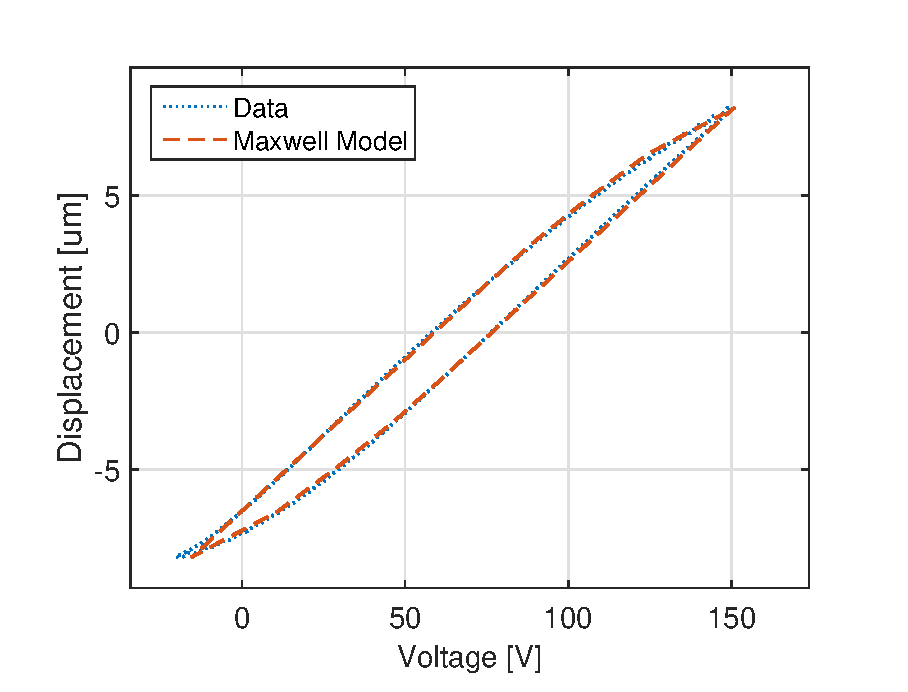
\includegraphics[width=0.7\textwidth]{fig/matlab/maxwell.eps}
  \caption{\label{fig:maxwell} The plot shows the model fit of the Maxwell slip model to the acquired hysteresis of the rotational stage. The fit has a mean squared error of 1.1464.}
\end{figure}

\begin{table}[h!]
  \centering
  \begin{tabular}{| l | l | l |}
    \hline
    $i$ & $k_i$ & $f_i$ \\ \hline
    1 & 4.53 & 3.69 \\
    2 & 0.90 & 1.46 \\
    3 & 1.01 & 2.47 \\
    4 & 0.36 & 1.16 \\
    5 & $1.49 \times 10^{-6}$ & $4.28 \times 10^{-6}$ \\
    6 & $2.89 \times 10^{-7}$ & $1.41 \times 10^{-6}$ \\
    7 & $1.59 \times 10^{-7}$ & $9.10 \times 10^{-7}$ \\
    8 & $1.39 \times 10^{-7}$ & $9.10 \times 10^{-7}$ \\
    9 & $2.28 \times 10^{-7}$ & $1.67 \times 10^{-6}$ \\
    10 & $4.58$ & 37.30 \\
    \hline
  \end{tabular}
  \caption{\label{tab:maxwell} Identified parameters of the Maxwell slip model.}
\end{table}

\subsection{Linear System Identification}
\label{sec:linsys}
The extracted linear dynamics have been identified as a $6^{th}$ order transfer function using a \abbrPRBS as excitation signal, allowing for a valid extraction from the nonlinear dynamics. The system transfer function has been derived in discrete-time using the System Identification Toolbox in Matlab. A more detail description of the procedure is available in \citep{ButcherController:2015}. Figure~\ref{fig:model} shows a comparison between the model and the real system in the frequency domain, where the Fast Fourier Transform (\abbrFFT) identification is calculated by taking the \abbrFFT of the output divided by the \abbrFFT of the input.
\begin{figure}[h]
  \centering
  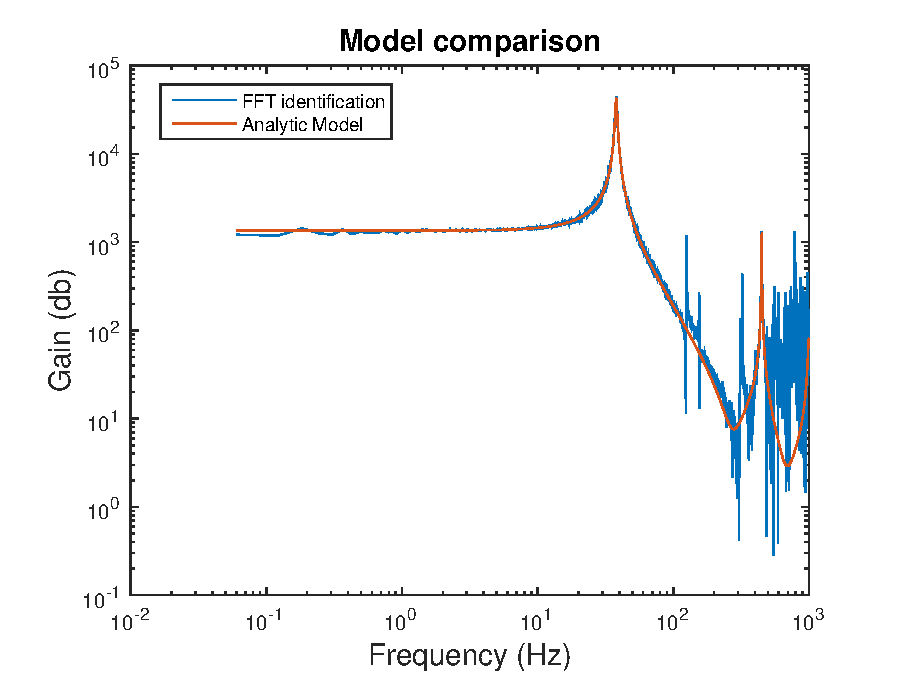
\includegraphics[width=0.7\textwidth]{fig/matlab/model.eps}
  \caption{\label{fig:model} The plot shows the model fit of a transfer function estimation with 5 zeros and 6 poles.}
\end{figure}
The transfer function of the model, discretized with a sampling time of \unit{0.5}{\milli\second}, is presented in \eqref{eq:tf}.

\begin{equation}
  \label{eq:tf}
  G(z) = \frac{21.05z^{-1} - 6.85z^{-2} + 8.52z^{-3} - 0.71z^{-4} + 9.30z^{-5}}{1344 - 2481z^{-1} + 1469z^{-2} + 21.64z^{-3} - 1767z^{-4} + 2084z^{-5} - 639.5z^{-6}}
\end{equation}

\FloatBarrier
\section{Present Control Approach}\label{sec:presentControlApproach}
The original controller for the rotational stage is a 2-\abbrDOF structure (feedback and prefilter). A schematic overview of the control loop is depicted in Figure~\ref{fig:present}, consisting of a controller block C, a prefilter F, a disturbance d and the linearized rotational stage $G = H^{-1}G_0$, where $G_0 = HG$ is the linear and nonlinear dynamics and $H^{-1}$ is the hysteresis compensator.

\begin{figure}[h]
  \centering %crop: left bottom right top
  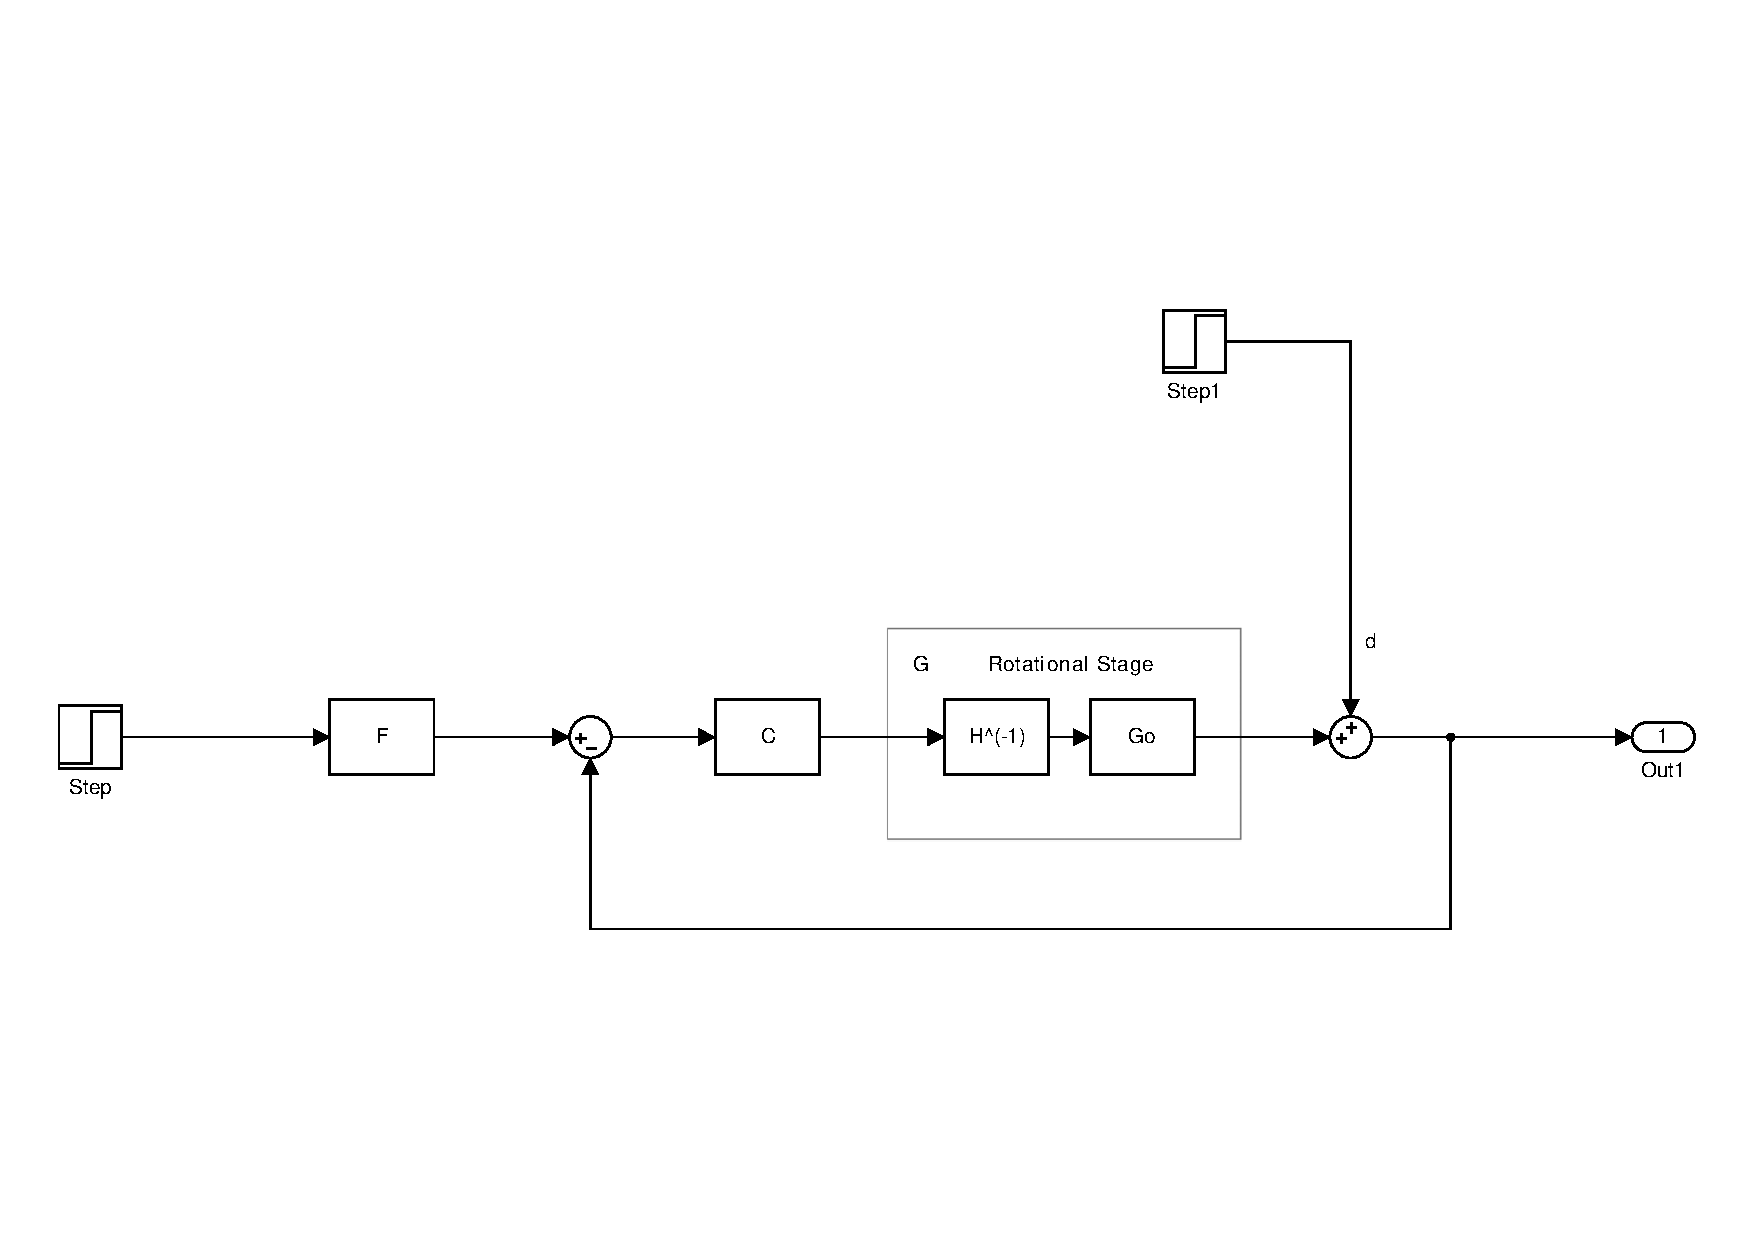
\includegraphics[width=1\textwidth, trim=4cm 3cm 2.1cm 10cm, clip=true]{fig/matlab/present_controller}
  \caption{\label{fig:present}Block diagram of the present control loop, inlcuding controller, prefilter and hysteresis compensator.}
\end{figure}

The controller block (C) is a series combination of a \abbrPID controller, notch filter and a lead filter, aiming to stabilize the system (\abbrPID), increase the sufficient phase margin (lead) and make the system more robust to high frequency oscillations (notch). Since the open loop bandwidth is relatively low, $f_b = 58 Hz$ according to Figure~\ref{fig:model}, it was decided to exclude cancellation of the first resonance peak in order to maintain the bandwidth as high as possible and to have sufficient attenuation of the resonance peak \citep{ButcherController:2015}. Finally, to enhance the tracking performance, a prefilter (F) was also added to the system. The PID controller, lead network, notch filter and prefilter are all presented below in \eqref{eq:controller}.

\begin{subequations}
  \label{eq:controller}
\begin{alignat}{2}
  \label{eq:pre}
  & F = \frac{0.0029z - 0.0029}{z^3 - 2.91z^2 + 2.816 z - 0.91} \\
  \label{eq:pid}
  & C_{PID} = \frac{0.47z^2 - 0.94z + 0.47}{z^2 - 1.78 z + 0.78} \\
  \label{eq:lead}
  & C_{lead} = \frac{4.20 z^2 - 7.72z + 3.55}{z^2 - 1.67z + 0.69} \\
  \label{eq:notch}
  & C_{notch} = \frac{0.28z^4 - 0.62z^3 + 0.75z^2 - 0.59z + 0.26}{z^4 - 1.95z^3 + 1.39z^2 - 0.40z + 0.039}
\end{alignat}
\end{subequations}

The effect of each filter can be seen in Figure~\ref{fig:opensys}, where the open loop system is plotted with one filter added at a time. One can see that the high resonance peak is mitigated after the notch filter have been added, that the lead filter rises the phase and that the \abbrPID controller provides good phase and gain margin. Also the closed loop system is presented in Figure~\ref{fig:closedsys}, proving that the prefilter increases the closed loop bandwidth. The final closed loop bandwidth is 9.7 Hz.

\begin{figure}[h!]
  \centering %crop: left bottom right top
  \subfloat[][\label{fig:opensys} Open loop]{
  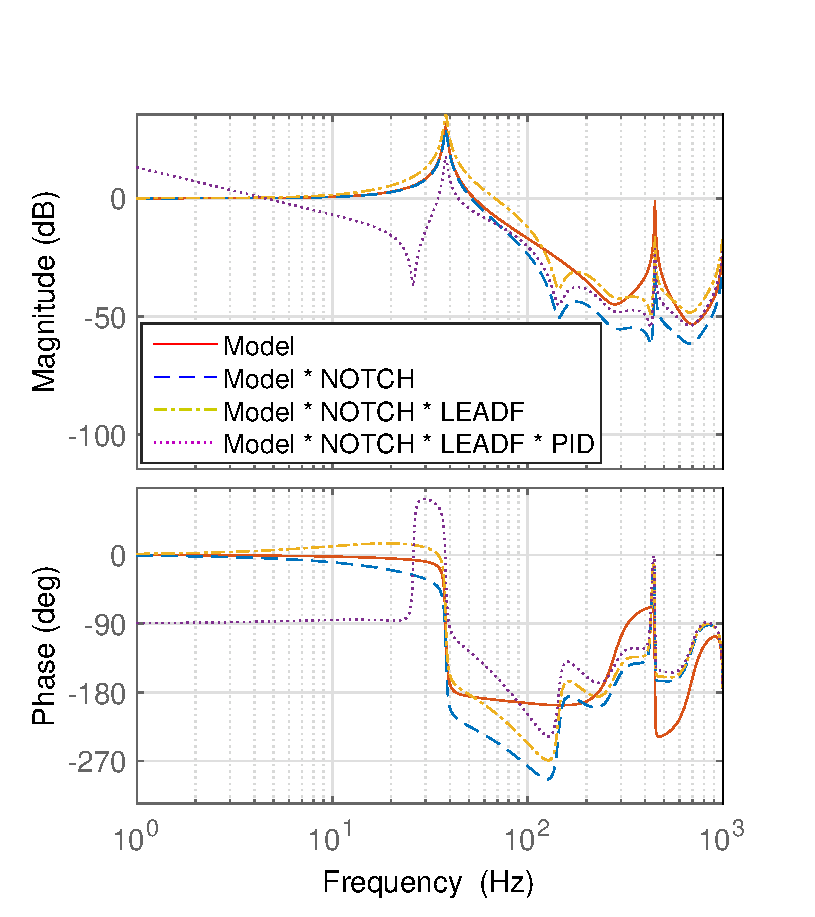
\includegraphics[width=0.46\textwidth, trim=0cm 0cm 1cm 0cm, clip=true]{fig/matlab/openloop_sys.eps}}
  \qquad
  \subfloat[][\label{fig:closedsys} Closed loop]{
  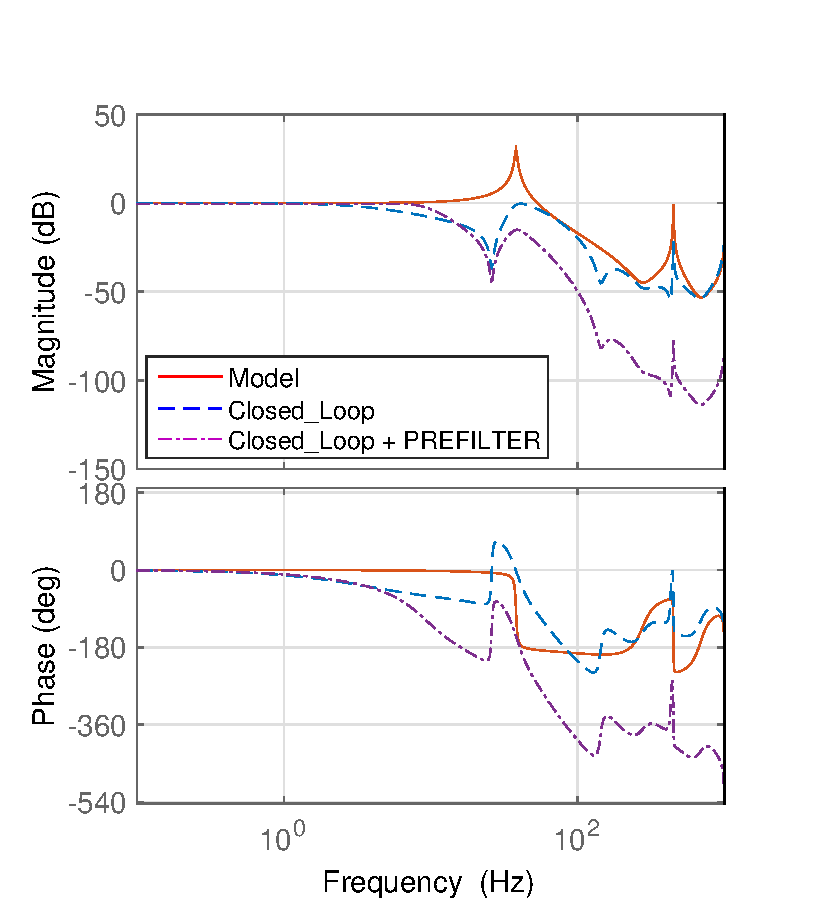
\includegraphics[width=0.46\textwidth, trim=0cm 0cm 1cm 0cm, clip=true]{fig/matlab/closedloop_sys.eps}}
  \caption{\label{fig:open_and_closed_sys} Illustration of controller effect. The effect of adding the different filters is shown in the open loop bode plot in (a) with the resulting closed loop system, with the open loop containing all filters, in (b). }
\end{figure}

% !TEX root = main.tex
\chapter{Modelling and System Identification}\label{cha:modelling}

% !TEX root = main.tex
\chapter{Modelling and System Identification}\label{cha:modelling}

% !TEX root = main.tex
%preliminära resultat som kan demonstreras vid halvtidskontroll
\chapter{Result}\label{cha:result}
This section describes future results that could be expected half way through the project.

\section{Control Approaches}
Half way through the project, all control approaches that have been identified should be presented here. Furthermore, all control approaches that at the time have been simulated will be presented with a schematic structure, transfer functions or state space model, a bode plot of the closed loop system and additional plots for illustration of the trajectory tracking capability and the robustness.

\section{Benchmark tests}
Benchmark tests will be carried out on all simulated control approaches and presented here. Comparisons between the new control approaches and the existing algorithm with respect to disturbance rejection, trajectory tracking and closed loop bandwidth will be illustrated in this section with plots and tables.

% !TEX root = main.tex
\chapter{Conclusion and Future work}\label{cha:conclusion}
This thesis has investigated in different control approaches aiming to improve the tracking capability of the rotational stage used in the UA9 collimation studies at \abbrCERN. The investigation showed that the \abbrIRC method can be used efficiently to attenuate the first resonance mode and increase the closed loop bandwidth. It also showed that the \abbrMRACPE can be used to adapt to the model changes and prevent instability. Furthermore it has shown that harmonic cancellation can be used to efficiently damp out known harmonic disturbances. Finally a feedforward harmonic cancellation method (\abbrRFDC) was implemented and proposed as an add-on control algorithm. This algorithm was first introduced for the control of hardware drives but has in this thesis shown to be effective with piezoelectric actuators and monolithic structures as well.

\section{Conclusions}
This results gathered during the simulations and the implementation of the \abbrRFDC are discussed below. The finding made in this thesis are presented with respect to the achieved results, highlighting theoretical and practical considerations.

\subsection{Simulations}
\subsubsection{Stand-alone control approaches}
The comparison presented in Section~\ref{sec:comparison} summarizes the simulation results. Looking at Table~\ref{tab:comp}, none of the control approaches are superior to another but the \abbrIRC is the most promising one with respect to the trade-off between tracking accuracy, sensitivity to model errors, stability issues and implementation considerations. The \abbrIRC handles severe model errors corresponding to a first resonance peak being moved from its original position in 38.1Hz to 22Hz and 67.2Hz, respectively. The model changes are by far more significant than the results presented in Figure~\ref{fig:different_angles}, depicting the model's yaw angular dependence, meaning that the \abbrIRC would be robust to these changes. Worth mentioning is also that the present controller has shown to be robust to the identified and more realistic model changes (the table only shows the resonance values where one approach becomes unstable).

In this context and for low angular rates, the adaptive controller has shown good results. However, the adaptive controller has shown drawbacks in many other aspects such as stability and disturbance rejection as outlined in the table. Instability can be caused if the controller has a too high gain with respect to the step size that is applied as input. This nonlinear phenomenon was observed in simulations without any saturation of the input signal, indicating that the amplitude dependent behavior shown in Figure~\ref{fig:step_adaptive} might be due to numerical errors. A higher sampling rate would, if not solve the problem completely, at least enhance the border to instability. Another way to maintain stability is to select the initial values more wisely to obtain a quicker convergence without increasing the gain. Figure~\ref{fig:periodic_resp} shows the adaptive performance of a periodic input, showing that the controller performs much better for the second period when the parameter is closer to their final value. Considering these issues, the adaptive controller might be better for being used as a secondary controller for long term parameter adaption, at least for operation in 2kHz.

The major advantage with the \abbrIRC is that it attenuates the first resonance peak, allowing for a higher bandwidth but also that this attenuation follows, at least in some extent, the changes in the resonance peak. The negative feedforward gain impacts on the placement of the interlacing zeros, but the placement is also highly dependent on the system itself, since it is in closed loop with the gain. With its higher bandwidth the \abbrIRC outperformed the present controller in tracking accuracy as shown in Aspect 3 in Table~\ref{tab:comp}. However, neither the present nor the \abbrIRC eliminates the constant ramp tracking error completely due to a non existing double integrator in the controller. A high bandwidth also implies in a controller that is more sensitive to measurement noise and to model errors in terms of stability, as shown in Figure~\ref{fig:model_dist_high_order}. Considering the fact that the yaw angle measurement is done by interfering with light in ultra high vacuum, there is no significant measurement error other than if the equipment would break down.

\subsubsection{Harmonic cancellation}
To increase the tracking accuracy even further, the \abbrIRC could be used in combination with a harmonics cancellation algorithm. The simulations in this thesis has shown that the \abbrRFDC could be a good candidate for canceling specific harmonic disturbances, especially the ones induced outside the bandwidth not reachable by the controller itself. In Table~\ref{tab:comp_h} the \abbrIMP might seem superior at a first glance but this is not the case. The \abbrIMP is directly inserted in the closed loop, affecting the closed loop system, deteriorating the sensitivity function and thereby amplifying disturbances with frequencies close to the cancellation frequency. This is not a suitable method for a system containing a lot of induced harmonics closely coupled together as seen in Figure~\ref{fig:dist_diff_speed}.

The other two cancellation methods are based on a feedforward approach and do not affect the closed loop system. With respect to cancellation effectiveness with induced model errors (Aspect 3 and 4 in Table~\ref{tab:comp_h}), the \abbrFDC is remarkable better than the \abbrRFDC. However, this result might be misleading, due to several reasons. Firstly, this approach requires a full model of the disturbance that has to be fed with a known input signal i.e. the disturbance must be known in quite a large extent. Secondly, the \abbrFDC performance is only evaluated over one step and only works with a low step rate as input. If the step rate is to high the response could be interfering with other step responses making the disturbance even harder to model. Nevertheless can it cancel environmental disturbances that do not originate from the system itself.

Considering the above with the goal to cancel out harmonic oscillations, the \abbrRFDC is the most preferable approach. It allows for cancellation of known harmonic disturbances while it only uses the angular measurement and the given output at the time to estimate the correct phase and amplitude of the disturbance. The observer converge time must be carefully estimated. In the simulations it was confirmed that the a quicker convergence implies in more noise added to the observed model, especially for high frequency models with frequencies close to the Nyquist frequency. The addition of a bandpass filter has not shown any increase of the cancellation performance. The problem lies in the fact that non modeled disturbances that enter the disturbance estimation become phase-shifted by the filter which lead to an amplification of its frequency components.

\subsection{Implementation}
The \abbrRFDC implementation showed good results, overall consistent with the results from the simulations. Cancellation was verified both in open and closed loop and with the selection of single and multiple disturbances. One important result is shown in Figure~\ref{fig:mult50no80}, where the 50Hz is canceled without affecting the 80Hz component. This also show that an environmental disturbance (not generated by a shaker), can be effectively reduced by this implementation. The environmental disturbances in the lab was much higher than the expected level of disturbance in the tunnel. This implied in a standard deviation varying between \unit{1}{\micro\radian} and \unit{10}{\micro\radian} in closed loop operation. Such a large varying standard deviation makes it difficult to compare 2 acquisitions that was not successively acquired directly after one another. Hence, the reduction of the yaw angle shown in for instance Figure~\ref{fig:yl_closedloop_80} should only be taken as an indication of the harmonic cancellation capability. This also explains the big difference between the open and closed loop performance, shown in Figure~\ref{fig:fft_openloop_80} and Figure~\ref{fig:fft_closedloop_80}, which in theory should have the same cancellation performance after the response has settled.

The implementation also showed an effect that was not captured in the simulations, i.e. the "beat effect" showing as an oscillation in the cancellation performance. This undesirable effect must be overcome before this algorithm can be implemented on the real controller that operates in the \abbrLHC tunnel. Solutions to mitigate this effect are discussed in the following section.

\section{Future work}
In the future, the tracking capability could be enhanced even further by combining some of the methods used in this thesis. For example to increase bandwidth and tracking capability the \abbrIRC could be implemented, and for the rejection of specific induced harmonics, the \abbrRFDC could be used without deteriorating the sensitivity to disturbances and model errors. Also an adaptive approach might be valuable to measure and adapt the controller parameters to long term effects such as thermal effects and aging of the piezoelectric actuator.

Improvement in the mechanical design could also be done. In fact, a new, high stiffness rotational stage has already been manufactured with the aim of increasing the stiffness of the system and thereby also extending the bandwidth, allowing for a more precise tracking and a better disturbance rejection. Even though it has a higher bandwidth than the previous stage, different angular and linear positions still changes the linear model drastically. The \abbrIRC is a promising control technique for handling these kind of model changes since it only uses a negative feedforward to damp out the first resonance peak and has no direct information of where the first resonance peak may be located. However, further investigation has to be carried out in order to gain a better knowledge about the controller robustness to high order model changes and techniques that can be used to be more robust to them.

To improve the already implemented \abbrRFDC method, several of adjustments can be made. For instance, a big drawback is that the frequencies that can be selected as subject for cancellation must have an integer number of periods that is a multiple of the sampling time. To achieve intersample disturbance rejection, a multi rate control technique with a control period shorter than the sampling period can be implemented, as proposed in \citep{fujimoto2009rro}. Another improvement would be to get rid of the beat effect. The effect could be mitigated by using some technique that regularly synchronizes the observed disturbance with the replicated one. One way could be to observe the disturbance at all the time and only use a few elements to synchronize the phase of the replicated disturbance. Another way could be to regularly create a new disturbance signal by updating the observed signal model, but how this technique would work in its full is left for future investigation.


% THESIS PLAN
% % !TEX root = main.tex
%en preliminär problemformulering satt i relation till litteraturbasen
\chapter{Introduction}\label{cha:intro}

\section{Background}
The piezoelectric effect is a phenomenon that arises in certain solid materials when an electric potential is generated in response to applied mechanical stress. The effect was first discovered by Jacques and Pierre Curie in 1880 when they found that applying pressure to a quarz crystal generates electrical potential. Today, the effect is commonly encountered in daily life and utilized in for example lighters, buzzers and loudspeakers.

Smart materials such as piezoelectric and magnetostrictive materials are nowadays commonly used in precision actuators due to their ability to convert electrical energy into mechanical energy. Piezoelectric materials have been commercially available for almost 45 years and have become indispensable for the nanopositioning industry \citep{Piezo:2008}. In cases where a relatively small displacement range is required (travel ranges up to \unit{500}{\micro\meter}) a piezo electric device is the actuator of choice due to its fast response, high resolution and its ability to generate large mechanical forces for small amounts of power in compact designs \citep{SurveyOfControlIssues:2007}.

High precision positioning systems are vital in e.g. scanning tunneling microscopes (\abbrSTM), atomic force microscopes (\abbrAFM) and in semiconductor lithography. In \abbrAFM, for instance, high precision positioning is required to control the vertical position of the scanning probe to keep the force constant between the sample surface and the probe tip. An topographical image of the sample is obtained by raster-scanning the probe over the sample surface and plotting the vertical displacement against the probe's x-y position. A positioning system that keeps the force constant down to an atomic-scale resolution is thus inevitable in order to obtain a high resolution image without damaging the sample \citep{SurveyOfControlIssues:2007}.

The Equipment Controls and Electronics section in the Engineering Department at \abbrCERN (European Organization for Nuclear Research) is developing a high precision positioning system for the control of a piezo-actuated rotational stage used in the UA9 Crystal Collimation study. The stage uses a piezo electric linear stack actuator to displace a flexible lever arm mechanism which generates the rotational movement.

\section{Purpose and Goal}
Crystalline solids have the ability to constrain the directions that particles take as they pass through, this is commonly called the "channelling" property. The UA9 collaboration at \abbrCERN is investigating how tiny bent crystals can help to steer particle beams in modern hadron colliders such as the Large Hadron Collider (\abbrLHC) \citep{WebsiteUA9:2016}. In high energy colliders, such as the \abbrLHC, particles tends to drift outwards creating a beam halo. These particles surrounding the beam, can be lost and cause damage to sensitive parts in the accelerator. By using bent crystals, halo particles can be efficiently extracted from the beam and collected by absorbers further away, reducing the complexity of the system. One major difficulty that aries is that the higher the energy of the particle, the lower the angular acceptance for channeling. Hence, a high precision positioning mechanism with a high angular accuracy is required. The rotational stage (with a range of \unit{20}{\milli\rad}) is of necessity to be able to track reference trajectories at ramp rates of \unit{100}{\micro\radianpersecond} and reject external disturbances to maintain a maximum tracking error of $\pm$\unit{1}{\micro\rad}.

This project aims to identify the possible control approaches that could be applicable to this problem to achieve the desired performance.

\section{Prospective challenges}
First of all, piezoelectric  actuators show strong nonlinear properties such as hysteresis and creep (drift), which have to be compensated for. Moreover, the mechanical flexural structure in combination with the piezo electric characteristics leads to a highly resonant structure, making it difficult to achieve the desired performance while operating the rotational stage within noisy environments with external disturbances such as ground vibrations.

Furthermore this rotational stage is attached to a linear stage which is composed by a leadscrew, a stepping motor and an axel. The linear movement adds additional perturbation to the rotational stage due to imperfections in the leadscrew and detent torque and stepping nature of the motor.

Finally the system dynamics also show linear position dependence requiring a controller that is robust to such variations.

\section{Related work}
One attempt to achieve the desired performance has already been made. The proposed controller, presented in \citep{ButcherController:2015} delivers reasonable performance but does not fulfill the requirements during movement. The authors proposes a PID controller in combination with a pre-filter, and a hysteresis compensator. The controller has shown high disturbance rejection at the first resonance peak as well as good tracking performance.

\section{Outline}
This thesis plan presents an overview of the thesis, including method, literature base and expected results. The method and work flow of the thesis as well as a comprehensive literature review is given in Chapter~\ref{cha:method}. In Chapter~\ref{cha:result} the results that can be expected half way through the project is discussed while a brief summary of the thesis can be found in Chapter~\ref{cha:conclusion}.

% % !TEX root = main.tex
% en preliminär beskrivning av angreppssätt
\chapter{Method}\label{cha:method}
This thesis will identify possible control approaches that could be applicable to the rotational stage at \abbrCERN in order to meet the performance requirements.
First of all, a brief analysis of the already developed controller will be done in order to point out the drawbacks and determine which controller qualities that have to be improved in order to achieved the desired performance during linear movement of the rotational stage. The main work will then consist of investigating different control approaches such as feedforward, H-infinity, iterative or state feedback control. The most promising approaches will be benchmarked in simulations and compared to the existing algorithm. Finally, the most promising alternative will be implemented and tested on the real rotational stage.

\section{Literature review}
Here follows a review of the preliminary literature base that will be used in this thesis. It will most likely be extended with more articles, papers and books during the work with this thesis.

\subsection*{\citep*{Biggio:2014} {\small \emph{- Memory characteristics of hysteresis and creep in multi-layer piezoelectric actuators: An experimental analysis}}}
The aim of this article is to provide an explanation of peculiar features of the piezoelectric actuator (\abbrPEA) response. It presents an experimental characterization of the nonlinear effects i.e. hysteresis and creep in a \abbrPEA. The authors find that both the instantaneous and delayed response of the PEA have hysteric dependence on the applied voltage level.
Moreover, they present experimental evidence for that the two observed hysteretic relationships share a common memory structure i.e. they are not truly independent nonlinear phenomenas.

\subsection*{\citep*{ButcherIdentification:2015}{\small \emph{- On the identification of Hammerstein systems in the presence of an input hysteretic nonlinearity with nonlocal memory: Piezoelectric actuators – an experimental case study}}}
This paper discusses the identification procedure of the linear dynamic part of piezo based actuators. A Hammerstein structure, consisting of a static (rate independent) hysteresis model with nonlocal memory (the current output does not only depend on the current input voltage but also on its history) and a linear dynamic model, is employed in order to model the hysteretic and dynamic behavior of the actuator.

The authors state that for the identification of the linear part of the actuator, a careful choice of the driving signal has to be made to avoid modifying the characteristics of the excitation. They show that a choice of a \abbrPBRS signal allows the decoupling of the identification of the linear and nonlinear part, since the nonlinear part only transforms the \abbrPBRS signal into another \abbrPBRS.

\subsection*{\citep*{ButcherController:2015} {\small \emph{- Controller Design and Verification for a Rotational Piezo-based Actuator for Accurate Positioning Applications in Noisy Environments}} }
This paper presents the modeling and controller design of a piezo actuated rotational stage operating in a noisy environment at CERN. The authors have adopted a Hammerstein structure, allowing them, in principal, to decouple the nonlinear hysteresis from the linear system dynamics. The extracted linear dynamics is identified as an OE system using several pseudo random binary signals (\abbrPBRS) as excitation signals. By adding different voltage biases to the PBRS it is also verified that the operating voltage point influences the identified transfer function (\abbrTF). The DC gain and the first resonance frequency and amplitude is affected due to the nonlinear piezo properties.

A 2-\abbrDOF controller (feedback and prefilter) and a hysteresis compensator are adopted in order to obtain the desired tracking and disturbance rejection. The proposed controller is designed as a series combination of a \abbrPID controller, a lead network and a 4\textsuperscript{th} order notch filter according to the quantitative feedback theorem (\abbrQFT). The proposed controller is experimentally tested and shows both disturbance rejection and good tracking capability.

\subsection*{\citep*{SurveyOfControlIssues:2007} {\small \emph{- A survey of control issues in nanopositioning}} }
This paper reviews the control-related research in nanopositioning, covering nanopositioning applications, actuators and sensors as well as control challenges. It focuses on piezoelectric actuators discussing both issues in control and different control techniques. Modeling techniques for the nonlinear effects i.e. creep and hysteresis as well as issues such as vibrations and modeling errors are presented in this work. Finally, different control schemes to mitigate the impact from these issues are reviewed such as feedback, forward, iterative and sensor less control.


\subsection*{\citep*{Piezo:2008} {\small \emph{- Piezoelectrics in Positioning, Tutorial on Piezotechnology in Nanopositioning Applications}} }
This tutorial by Physik Instrumente (PI) gives the reader an overview of the fundamentals of piezoelectricity, piezomechanics and piezo actuators as well as detailed information regarding control approaches, environmental dependencies and design of piezoelectric positioning drives/systems. The electrical, mechanical and thermal behavior of piezoelectric actuators is described by basic equations presented in this paper. Several methods to improve the piezo dynamics are also discussed, such as linearization, signal preshaping and InputShaping® which is a patented real-time feedforward technology.

\subsection*{\citep*{FlemingLeang:2014} {\small \emph{- Design, Modeling and Control of Nanopositioning Systems}} }
This book covers the complete design cycle of nanopositioning systems. Some relevant chapters with respect to this thesis are Hysteresis Modeling and Control, Noise in Nanopositioning and Mechanical Design: Flexure-Based Nanopositioners.


\section{Timeplan}
%en tidplan för examensarbetets genomförande inklusive planerade datum för halvtidskontroll och framläggning
Figure~\ref{fig:timeplan} shows the timeplan for the master thesis project. \emph{HP} and \emph{FP} stands for halftime presentation and fulltime presentation, respectively. In addition to the master thesis work, some hardware testing will be carried out from time to time, throughout the whole thesis period.

\begin{figure}[h] %tbp
 \centering %crop: left bottom right top
 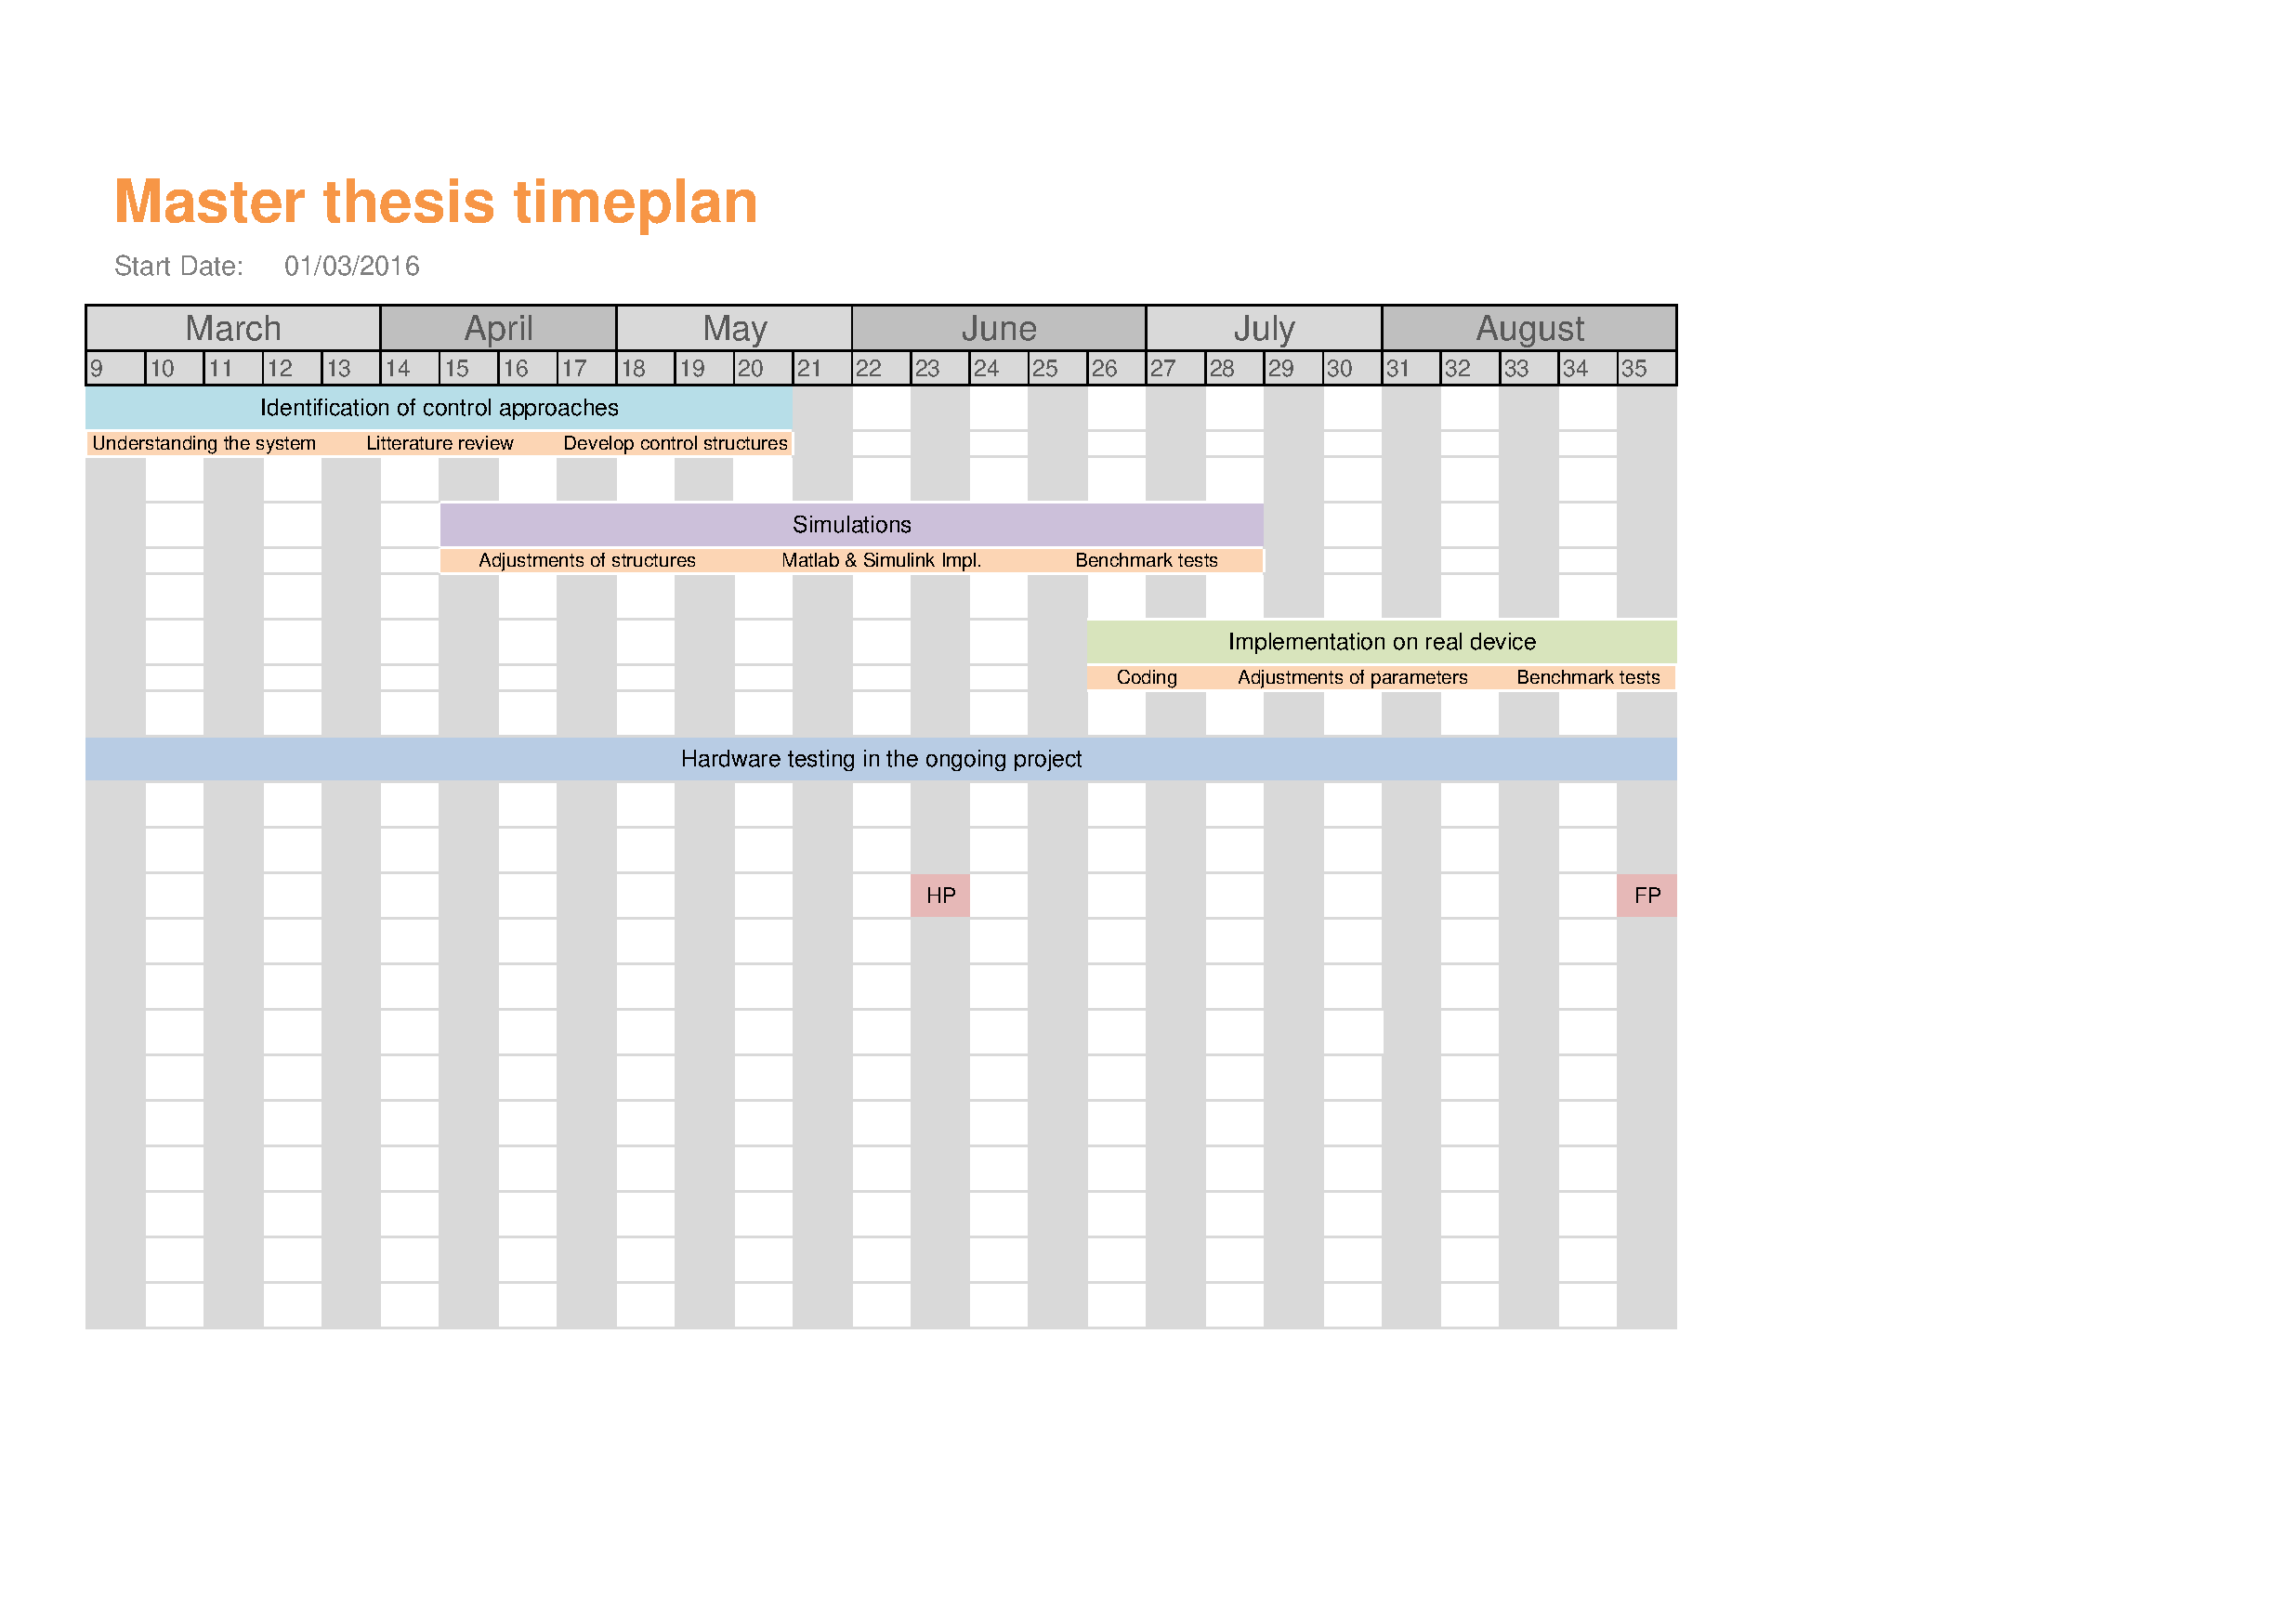
\includegraphics[trim=1cm 12cm 5cm 5.5cm, clip=true, scale=0.42]{fig/timeplan}
 \caption{\label{fig:timeplan}%
 Master Thesis timeplan}
 \end{figure}

% % !TEX root = main.tex
%preliminära resultat som kan demonstreras vid halvtidskontroll
\chapter{Result}\label{cha:result}
This section describes future results that could be expected half way through the project.

\section{Control Approaches}
Half way through the project, all control approaches that have been identified should be presented here. Furthermore, all control approaches that at the time have been simulated will be presented with a schematic structure, transfer functions or state space model, a bode plot of the closed loop system and additional plots for illustration of the trajectory tracking capability and the robustness.

\section{Benchmark tests}
Benchmark tests will be carried out on all simulated control approaches and presented here. Comparisons between the new control approaches and the existing algorithm with respect to disturbance rejection, trajectory tracking and closed loop bandwidth will be illustrated in this section with plots and tables.

% %Sätt av ett kort kapitel sist i rapporten till att avrunda och föreslå rikningar för framtida utveckling av arbetet.
% !TEX root = main.tex
\chapter{Conclusion}\label{cha:conclusion}

This thesis aims to identify, simulate and implement a suitable control approach for a piezo actuated rotational stage at \abbrCERN. The rotational stage is to be used within the UA9 project to position a bent crystal (which will steer particle beams) with a high accuracy. Several control approaches will be simulated in order to find a controller that meet the requirements. The best performing approach will be implemented and tested on the real device. 


\part*{Appendix}
\appendix
%
\chapter{definitions}\label{cha:definition}

\section{Test}

\clearemptydoublepage

\backmatter

\bibliography{IEEEfull,myrefs}

\printindex

\end{document}
